% +------------------------------------------------------------------------+
% | CGAL Reference Manual:  wrapper.tex
% +------------------------------------------------------------------------+
% | Main TeX file for testing CGAL packages.
% +------------------------------------------------------------------------+

\documentclass{book}


%%%%%%%%%%%%%%%%%%%%%%%%%%%%%%%%%%%%%%%%%%%%%%%%%%%%%%%%%%%%%%%%%%%%%%%
%\usepackage{cprog}
%\usepackage{cc_manual}
%\usepackage{cc_manual_index}
%\usepackage{amssymb}
%\usepackage{graphicx}
%\usepackage{path}
%\usepackage{ipe}

%% page dimensions
%% ---------------
%% The page dimensions are compulsory and may not be changed in main.tex.

%\textwidth 15.6cm 
%\textheight 23 cm
%\topmargin -14mm       
%\evensidemargin 3mm 
%\oddsidemargin 3mm

%% default column layout
%% ---------------------
%% This is the recommended layout. It may be changed inside main.tex.

%\newcommand{\cgalColumnLayout}{\ccTexHtml{%
%    \ccSetThreeColumns{Oriented_side}{}{\hspace*{8.5cm}}
%    \ccPropagateThreeToTwoColumns}{}}

%\sloppy

%\begin{document}

%\cgalColumnLayout
%%\tableofcontents
%% // ============================================================================
%//
%// Copyright (c) 1999 The CGAL Consortium
%//
%// This software and related documentation is part of an INTERNAL release
%// of the Computational Geometry Algorithms Library (CGAL). It is not
%// intended for general use.
%//
%// ----------------------------------------------------------------------------
%//
%// release       :
%// release_date  :
%//
%// file          : /doc_tex/basic/Triangulation3/Triangulation3.tex
%// revision      : $Revision$
%//
%// author(s)     : Monique Teillaud <Monique.Teillaud@sophia.inria.fr>
%//
%// coordinator   : INRIA Sophia Antipolis (Mariette Yvinec <Mariette.Yvinec@sophia.inria.fr>)
%//
%//============================================================================
\chapter{Triangulation in 3D}
\label{chapter-Triangulation3}
\begin{ccTexOnly}
\vspace*{-2cm}
\includegraphics{grille.eps} \hspace*{2cm} 
\includegraphics{sphere.eps} 
\end{ccTexOnly}
\begin{ccHtmlOnly}
<img border=0 src="./sphere.gif" align=center>
<img border=0 src="./grille.gif" align=center>
\end{ccHtmlOnly}
\section{Introduction}
\label{Triangulation3-sec-intro}
\subsection{Definition}
\label{Triangulation3-sec-def}
A three-dimensional triangulation is a three-dimensional simplicial
complex, pure connected and without singularities. (See
\cite{by-ag-98} or Chapter~\ref{I1_Chapter_Triangulations}.) Its
cells ($3$-faces) are such that two cells either do not intersect or
share a common facet ($2$-face), edge ($1$-face) or vertex ($0$-face).

The basic 3D-triangulation class of \cgal\ is primarily designed to
represent the triangulations of a set of points $A$ in $\R^3$.  It can
be viewed as a partition of the convex hull of {$A$} into tetrahedra
whose vertices are the points of {$A$}.  Together with the unbounded
cell having the convex hull boundary as its frontier, the triangulation
forms a partition of $\R^3$.

In order to deal
only with tetrahedra, which is convenient for many applications, the
unbounded cell can be subdivided into tetrahedra by considering that
each convex hull facet is incident to an \ccc{infinite cell} having as
fourth vertex an auxiliary vertex called the \ccc{infinite vertex}.  In
that way, each facet is incident to exactly two cells and special cases
at the boundary of the convex hull are simple to deal with.

The class \ccc{Triangulation_3<Triangulation_traits_3,Tds_3>} of \cgal\ implements this
point of view and therefore considers the triangulation of the set
of points as a set of finite and infinite tetrahedra.  Notice that the
infinite vertex has no significant coordinates and that no
geometric predicate can be applied on it.

A triangulation is a collection of vertices and cells that are linked
together through incidence and adjacency relations. Each cell gives
access to its four incident vertices and to its four adjacent
cells. Each vertex gives access to one of its incident cells.

The four vertices of a cell are indexed with 0, 1, 2 and 3 in positive
orientation, the positive orientation being defined by the orientation
of the underlying Euclidean space $\R^3$. The neighbors of a cell are also
indexed with 0, 1, 2, 3 in such a way that the neighbor indexed by $i$
is opposite to the vertex with the same index. See
Figure~\ref{Triangulation3-fig-orient}.

\begin{figure}[htbp]
\begin{ccTexOnly}
\begin{center} 
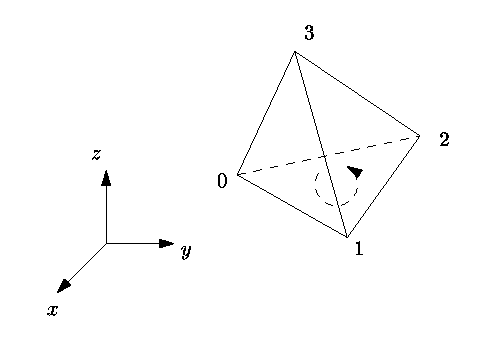
\includegraphics{orient.eps} 
\end{center}
\end{ccTexOnly}
\caption{Orientation of a cell (3-dimensional case).
\label{Triangulation3-fig-orient}}
\begin{ccHtmlOnly}
<CENTER>
<img border=0 src="./orient.gif" align=center alt="Orientation of a cell 
(3-dimensional case)">
</CENTER>
\end{ccHtmlOnly}
\end{figure} 

As in the underlying combinatorial triangulation (see
Chapter~\ref{chapter-TDS3}), edges ($1$-faces) and facets ($2$-faces)
are not explicitly 
represented: a facet is given by a cell and an index (the facet
\ccc{i} of a cell \ccc{c} is the facet of \ccc{c} that is opposite to
the vertex with index \ccc{i}) and an edge is given by a cell and two
indices (the edge \ccc{(i,j)} of a cell \ccc{c} is the edge whose
endpoints are the vertices of \ccc{c} with indices \ccc{i} and
\ccc{j}). See Figure~\ref{TDS3-fig-repres}.  

\subsection{Degenerate Dimensions}
\label{Triangulation3-sec-degen_dim}

The class \ccc{Triangulation_3<Triangulation_traits_3,Tds_3>} can also deal with
triangulations whose dimension is less than~3. A triangulation of a
set of points in $\R^d$ covers the whole space $\R^d$ and consists of
cells having $d+1$ vertices: some of them are infinite, they are
obtained by linking the additional infinite vertex to each facet of
the convex hull of the points.
\begin{itemize}
\item {} \emph{dimension 2:} when a triangulation only contains
coplanar points (which is the case when there are only three points), 
it consists of triangular faces.
\item {} \emph{dimension 1:} the triangulation contains only collinear 
points (which is the case when there are only two points), it consists
of edges.
\item {} \emph{dimension 0:} the triangulation contains only one
finite point.
\item {} \emph{dimension -1:} this is a convention to handle the case
when the only vertex of the triangulation is the infinite one.
\end{itemize} 

The same cell class is used in all cases: triangular faces in
2D can be considered as degenerate cells, having only three vertices
(resp. neighbors)
numbered $(0,1,2)$, and one $NULL$ vertex (resp. neighbor);
edges in 1D have only two vertices (resp. neighbors) numbered $0$ and $1$. 

The implicit representation of facets (resp. edges) still holds
for degenerate dimensions (\textit{i.e.}dimensions $<3$) : in
dimension~2, each cell has only one facet of index 3, and 3 edges
$(0,1)$, $(1,2)$ and $(2,0)$; in dimension~1, each cell has one edge
$(0,1)$.  

\subsection{Validity}
\label{Triangulation3-sec-Valid}

A triangulation of $\R^3$ is said to be \ccc{locally valid} iff

{\bf (a)-(b)} Its underlying combinatorial graph, the triangulation
data structure, is \ccc{locally valid} 
(see Section~\ref{TDS3-sec-Valid} of Chapter~\ref{chapter-TDS3})\\
{\bf (c)} Any cell has its vertices ordered according to positive
orientation. See Figure~\ref{Triangulation3-fig-orient}.

When the triangulation is degenerated into a triangulation of
dimension~2, the  geometric validity reduces to:

{\bf (c-2D)} For any two adjacent triangles $(u,v,w_1)$ and $(u,v,w_2)$ with
common edge $(u,v)$, $w_1$ and $w_2$ lie on opposite sides of $(u,v)$
in the plane.

When all the points are collinear, this condition becomes:

{\bf (c-1D)} For any two adjacent edges $(u,v)$ and $(v,w)$, $u$ and
$w$ lie on opposite sides of the common vertex $v$ on the line.

The \ccc{is_valid()} method provided by \cgal\ checks the local
validity of a given triangulation. This does not always
ensure global validity \cite{mnssssu-cgpvg-96,dlpt-ccpps-98} but it is 
sufficient for practical cases.

\section{Software Design}
\label{Triangulation3-sec-design}

The class \ccc{Triangulation_3<Triangulation_traits_3,Tds_3>} is designed to be used as 
a layer upon a 3D-triangulation data structure as presented in 
Section~\ref{TDS3-sec-design} of Chapter~\ref{chapter-TDS3}.
It provides high level geometric operations such as location of a point
in the triangulation and insertion of a point, and is responsible for
the geometric validity. This class is parameterized by two classes:
\begin{itemize}
\item {} the \textbf{geometric traits} class, where the user can
specify the type of points to use as well as the elementary
operations on them (predicates,\ldots). The concept of such a class is
introduced in Section~\ref{Triangulation3-sec-Traits} and described in 
\ccRefPage{Triangulation_traits_3} and a
model is provided by \cgal\
(see \ccRefPage{CGAL::Triangulation_geom_traits_3<R>} and 
\ccRefPage{CGAL::Regular_triangulation_euclidean_traits_3<R,Weight>}).
\item {} the \textbf{triangulation data structure} class of the middle level, 
described in Chapter~\ref{chapter-TDS3}.
\end{itemize}	

Delaunay triangulations as well as hierarchical Delaunay triangulations
\cite{d-iirdt-98} are also implemented in the package: 
\ccc{Delaunay_triangulation_3<Triangulation_traits_3,Tds_3>} inherits from 
\ccc{Triangulation_3<Triangulation_traits_3,Tds_3>} and 
\ccc{Delaunay_hierarchic_triangulation_3<Triangulation_traits_3,Tds_3>} inherits from 
\ccc{Delaunay_triangulation_3<Triangulation_traits_3,Tds_3>}. \textit{(Hierarchical
Delaunay triangulations are not yet implemented.)} 

\ccc{Triangulation_3<Triangulation_traits_3,Tds_3>} derives from
\ccc{Triangulation_utils_3<Triangulation_traits_3,Tds_3>}, 
which defines a set of tools
working on the indices of vertices in cells 
(\ccRefPage{CGAL::Triangulation_utils_3}). 

\subsection{Basic Triangulation}

\ccc{Triangulation_3<Triangulation_traits_3,Tds_3>} expects a model of a 
\textit{geometric traits class} as its first template argument and a model 
of a \textit{triangulation data structure} as its second argument. The
requirements and defaults for these classes are described in
\ccRefPage{Triangulation_traits_3},
\ccRefPage{CGAL::Triangulation_geom_traits_3<R>} and
\ccRefPage{CGAL::Regular_triangulation_euclidean_traits_3<R,Weight>}.

%\subsection{The Vertex of a Triangulation} 
%\label{Triangulation3-sec-class-Vertex}

%\begin{ccClassTemplate}{Triangulation_vertex_3<Triangulation_traits_3,Tds_3>}
%\ccCreationVariable{v}

%\ccDefinition
%The vertex stores a point and gives access to an incident face of
%maximal dimension.
%	\end{ccClassTemplate} 

%\subsection{The Cell of a Triangulation} 
%\label{Triangulation3-sec-class-Cell}

%\begin{ccClassTemplate}{Triangulation_cell_3<Triangulation_traits_3,Tds_3>}
%\ccCreationVariable{c}

%\ccDefinition

%A cell of a triangulation gives access to its four vertices indexed 0,
%1, 2, and 3 in positive orientation and to its four adjacent cells, also
%called neighbors. The neighbors are indexed in such a way that neighbor
%$i$ lies opposite to vertex $i$.

%In degenerate dimensions, cells are used to store faces of maximal
%dimension: (Section~\ref{Triangulation3-sec-degen_dim}).
%	\end{ccClassTemplate} 

\subsection{Delaunay Triangulation} 

The class \ccc{Delaunay_triangulation_3<Triangulation_traits_3,Tds_3>}
represents a three-dimensional Delaunay triangulation. 

\subsection{Hierarchic Delaunay Triangulation} 
(See~\cite{d-iirdt-98}.)
\ccc{Delaunay_hierarchic_triangulation_3<Triangulation_traits_3,Tds_3>}
\textit{Not yet implemented}

\subsection{Regular Triangulation} 
\label{Triangulation3-sec-class-Regulartriangulation}

\ccc{Regular_triangulation_3<Triangulation_traits_3,Tds_3>} implements
regular triangulations.

Let ${S}^{(w)}$ be a set of weighted points in $\R^3$. Let
${p}^{(w)}=(p,w_p), p\in\R^3, w_p\in\R$ and 
${z}^{(w)}=(z,w_z), z\in\R^3, w_z\in\R$ be two weighted points. 
A weighted point
${p}^{(w)}=(p,w_p)$ can also be seen as a sphere of center $p$ and
radius $w_p$. 
The \textit{power product} between ${p}^{(w)}$ and ${z}^{(w)}$ is
defined as 
\[\Pi({p}^{(w)},{z}^{(w)}) = {\|{p-z}\|^2-w_p^2-w_z^2}\]
where $\|{p-z}\|$ is the Euclidean distance between $p$ and $z$. 
 ${p}^{(w)}$ and ${z}^{(w)}$
are said to be \textit{orthogonal} if $\Pi{({p}^{(w)}-{z}^{(w)})}
= 0$ (see Figure~\ref{Triangulation3-fig-ortho}).

\begin{figure}[htbp]
\begin{ccTexOnly}
\begin{center} 
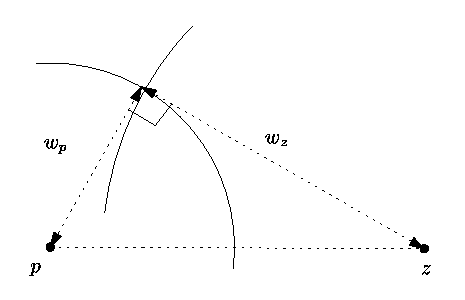
\includegraphics{ortho.eps} 
\end{center}
\end{ccTexOnly}
\caption{Orthogonal weighted points (picture in 2D).
\label{Triangulation3-fig-ortho}}
\begin{ccHtmlOnly}
<CENTER>
<img border=0 src="./ortho.gif" align=center alt="Orthogonal weighted
points (picture in 2D)"> 
</CENTER>
\end{ccHtmlOnly}
\end{figure} 

Four weighted points have a unique common orthogonal weighted point called
the \textit{power sphere}. A sphere ${z}^{(w)}$ is said to be
\textit{regular} if $\forall {p}^{(w)}\in{S}^{(w)},
\Pi{({p}^{(w)}-{z}^{(w)})}\geq 0$.

A triangulation of ${S}^{(w)}$ is \textit{regular} if the power spheres
of all simplices are regular. 

The regular triangulation of
${S}^{(w)}$ is in fact the projection onto $\R^3$ of the convex hull 
of the four-dimensional points $(p,\|p-O\|^2-w_p),$ for
${p}^{(w)}=(p,w_p)\in{S}^{(w)}$. 
Note that all points of ${S}^{(w)}$ do not
necessarily appear as vertices of the regular
triangulation. To know more about regular triangulations, see for
example \cite{es-itfwr-96}. 

When all weights are 0, power spheres are nothing more than
circumscribing spheres, and the regular triangulation is exactly the
Delaunay triangulation.

We will call the weighted point orthogonal to three weighted points in
the plane defined by these three points the \textit{power circle}. The
\textit{power segment} will denote the weighted point orthogonal to
two weighted points on the line defined by these two points.

To simplify notation, $p$ will often denote in the sequel either the
point $p\in\R^3$ or the weighted point ${p}^{(w)}=(p,w_p)$.

%\section{A Class of Tools \protect\ccc{Triangulation_utils_3}} 
%\section{A Class of Tools}
%\label{Triangulation3-sec-class-Utils}

%\begin{ccClass}{Triangulation_utils_3}
%The class \ccClassName\ defines operations on the indices of vertices
%and neighbors within a cell. These operations are used in
%\ccc{Triangulation_3.h},
%\ccc{Triangulation_data_structure_3.h},
%\ccc{Triangulation_ds_cell_3.h},
%\ccc{Triangulation_ds_circulators_3.h}. These classes inherit from
%\ccClassName\ so that they can use its methods.
%\end{ccClass}




%\section{Debugging}

%	\subsection{Pretty print}	
% \textit{to be written}

%	\subsection{Debugging with handles} 
%Most debuggers cannot understand \ccc{handles} well. Under the
%debugger, an instruction such as

%\texttt{(dbx) print -r c->vertex(0)}

%where \ccc{c} is a \ccc{Cell_handle}, is answered by:

%\texttt{can't find field "vertex" in "c"}

%To work around this problem, two functions have been defined to transform 
%\ccc{handles} into usual $C^{++}$ pointers for debugging purposes.

%\ccFunction{template <class Triangulation_traits_3, class Tds_3>
%	Triangulation_vertex_3<Triangulation_traits_3,Tds_3> * 
%debug(const Triangulation_vertex_handle_3<Triangulation_traits_3,Tds_3> v);}
%{}

%\ccFunction{template <class Triangulation_traits_3, class Tds_3>
%	Triangulation_cell_3<Triangulation_traits_3,Tds_3> * 
%	debug(const Triangulation_cell_handle_3<Triangulation_traits_3,Tds_3>
%c);}
%{}

%This allows the following:\\
%\texttt{(dbx) print -r CGAL\_debug(c)->vertex(0)\\
%CGAL\_debug(c)->vertex(0) = \{\\\
%\ldots\\
%\} }

\subsection{The Geometric Traits}
\label{Triangulation3-sec-Traits}

The first template parameter of the triangulation class
\ccc{Triangulation_3<Triangulation_traits_3,Tds_3>} of \cgal\ is the geometric traits class.

The geometric traits class must define the geometric
objects (points, segments, triangles and tetrahedra) forming the
triangulation together with a few geometric predicates on these objects:
equality, coordinate comparison, orientation in space, orientation
in case of coplanar points, and collinearity tests.

In addition to the requirements described before, the geometric traits
class of a Delaunay triangulation must define predicates for the
\textit{empty sphere property}.

To be used as the traits class for the regular triangulation provided
by \cgal, a class must provide definitions for the \textit{power tests}.
(See Section~\ref{Triangulation3-sec-class-Regulartriangulation}.)
	
\cgal\ provides a predefined geometric traits class 
\ccc{Triangulation_geom_traits_3<R>} using the kernel
geometric objects and predicates.
This class is templated with a representation class.

The traits class \ccClassTemplateName\ is designed to deal with \cgal\ three
dimensional points. It supplies the user with all
the functionalities described in
\ccRefPage{Triangulation_traits_3}.
So, it can be used as a default traits
class for \ccc{Triangulation_3<Triangulation_traits_3,Tds_3>},
\ccc{Delaunay_triangulation_3<Triangulation_traits_3,Tds_3>} and
\ccc{Delaunay_hierarchic_triangulation_3<Triangulation_traits_3,Tds_3>}.

\ccc{Regular_triangulation_euclidean_traits_3<R,Weight>} is a traits class 
 designed to be used by the class
\ccc{Regular_triangulation_3<Triangulation_traits_3,Tds_3>}. It provides
\ccc{Weighted_point}, a class for weighted points
provided by the class, which derives from the \cgal\ three dimensional
point class. It supplies
the user with all the functionalities 
described in \ccRefPage{Triangulation_traits_3}.
 It can be used as a default traits
class for \ccc{Regular_triangulation_3<Triangulation_traits_3,Tds_3>}.

%		\subsection{Weighted point}	
%		\label{Triangulation3-sec-class-Weightedpoints}

%		\subsubsection{Concept for a weighted point}

%The weighted point class is needed by 
%\ccc{Regular_triangulation_euclidean_traits_3}. 


%		\subsubsection{Model of weighted point} 

%		\begin{ccClassTemplate}{Weighted_point<Point,Weight>}
%This class provides \ccc{Regular_triangulation_euclidean_traits_3}
%with all the required functionalities.

%\ccInclude{CGAL/Weighted_point.h}

%\ccInheritsFrom{\ccc{Point} (the template parameter) }

%		\end{ccClassTemplate}

\subsection{The Triangulation Data Structure Parameter}
\label{Triangulation3-sec-tds}

The second template parameter of the basic triangulation class
\ccc{Triangulation_3<Triangulation_traits_3,Tds_3>} is a triangulation 
data structure class.  This class can be seen as a container for the
cells and vertices maintaining incidence and adjacency relations (see
Chapter~\ref{chapter-TDS3}).  A model of this triangulation data
structure is \ccc{Triangulation_data_structure_3} 
(\ccRefPage{CGAL::Triangulation_data_structure_3<Vb,Cb>}).

\section{Examples}
\label{Triangulation3-sec-examples}
This example shows the incremental construction of a 3D triangulation, 
the location of a point, and how to manipulate elementary operations
on indices in a cell.

\begin{verbatim}
#include <CGAL/basic.h>

#include <iostream>

#include <list>
#include <vector>

#include <CGAL/Cartesian.h>

#include <CGAL/Triangulation_cell_base_3.h>
#include <CGAL/Triangulation_vertex_base_3.h>
#include <CGAL/Triangulation_data_structure_3.h>
#include <CGAL/Triangulation_geom_traits_3.h>
#include <CGAL/Triangulation_3.h>

typedef CGAL::Cartesian<double>  Rep;

typedef CGAL::Triangulation_geom_traits_3<Rep> Gt;
typedef CGAL::Triangulation_vertex_base_3<Gt> Vb;
typedef CGAL::Triangulation_cell_base_3<Gt>  Cb;

typedef CGAL::Triangulation_data_structure_3<Vb,Cb> TDS;
typedef CGAL::Triangulation_3<Gt,TDS> Triangulation;

typedef typename Triangulation::Cell_handle Cell_handle;
typedef typename Triangulation::Vertex_handle Vertex_handle;
typedef typename Triangulation::Locate_type Locate_type;

typedef Gt::Point Point;

int main(int argc, char* argv[])
{

  Triangulation T;

  // insertion from a list :
  std::list<Point> L;
  L.push_front(Point(0,0,0));
  L.push_front(Point(1,0,0));
  L.push_front(Point(0,1,0));

  int n = T.insert(L.begin(), L.end());

  // insertion from a vector :
  std::vector<Point> V(3);
  V[0] = Point(0,0,1);
  V[1] = Point(1,1,1);
  V[2] = Point(2,2,2);

  n = n + T.insert(V.begin(), V.end());

  // 6 points have been inserted :
  assert( n == 6 );

  // checking validity of T :
  assert( T.is_valid(false) );

  Locate_type lt;
  int li, lj;
  Point p(0,0,0);
  Cell_handle c = T.locate(p, lt, li, lj);
  // p is the vertex of c of index li :
  assert( lt == Triangulation::VERTEX );
  assert(  c->vertex(li)->point() == p );

  Vertex_handle v = c->vertex( (li+1)&3 );
  // v is another vertex of c
  Cell_handle nc = c->neighbor(li);
  // nc = neighbor of c opposite to the vertex associated with p
  // nc must have vertex v :
  int nli;
  assert( nc->has_vertex( v, nli ) );
  // nli is the index of v in nc

  std::ofstream oFileT("output",ios::out);
  // writing file output; 
  oFileT << T; 

  return 0;
}
\end{verbatim}


%% =============================================================================
% The CGAL Reference Manual
% Chapter: Optimisation
% -----------------------------------------------------------------------------
% file  : doc_tex/basic/Optimisation/main.tex
% author: Bernd G�rtner, Sven Sch�nherr (sven@inf.fu-berlin.de)
% -----------------------------------------------------------------------------
% $Revision$
% $Date$
% =============================================================================

\newcommand{\linebreakByHand}{\ccTexHtml{\\}{}}
\newcommand{\SaveSpaceByHand}{}  %%%% [2]{\ccTexHtml{#1}{#2}}

\chapter{Geometric Optimisation} \label{Optimisation}
\RCSdefDate{\OptRCSDate}{$Date$}

\ccChapterRelease{Release: 2.0 \ccTexHtml{\quad}{ , } \OptRCSDate}

\ccChapterAuthor{Bernd G{\"a}rtner}\ccTexHtml{\\}{<br>}
\ccChapterAuthor{Michael Hoffmann}\ccTexHtml{\\}{<br>}
\ccChapterAuthor{Sven Sch{\"o}nherr}

\ccTexHtml{\thispagestyle{empty}}{}

\begin{ccTexOnly}\section*{Introduction}\end{ccTexOnly}
\begin{ccHtmlOnly}<H2>Introduction</H2><P>\end{ccHtmlOnly}

This chapter describes routines for solving geometric optimisation problems.
The first two sections contain algorithms for computing and updating the
smallest enclosing circle (Section~\ref{sec:smallest_enclosing_circles})
resp.\ ellipse (Section~\ref{sec:smallest_enclosing_ellipses}) of a finite
point set.  Formally, the `smallest enclosing circle' is the boundary of the
closed disk of minimum area covering the point set. It is known that this
disk is unique.  We usually identify the disk with its bounding circle,
allowing us to talk about points being on the boundary of the circle, etc.
The same holds for the smallest enclosing ellipse. These algorithms work in
an incremental manner. They are implemented as semi-dynamic data structures,
thus allowing to insert points while maintaining the smallest enclosing
circle resp.\ ellipse.

The remaining sections describe algorithms for searching in matrices with
specific properties and some applications. In particular, there are
general implementations of
\begin{itemize}
  \item monotone matrix search (see Section~\ref{secMonotoneMatrixSearch}),
    which can be applied to compute
    \begin{itemize}
      \item extremal polygons of a convex polygon
        (see Section~\ref{secComputingExtremalPolygons}) \textit{or}
      \item all furthest neighbors for the vertices of a convex polygon
        (see Section~\ref{secAllFurthestNeighbors}),
    \end{itemize}
  \item and sorted matrix search (see Section~\ref{secSortedMatrixSearch}),
    which can be used to compute the $p$-centers of a planar point set
    (see Section~\ref{sec_RectangularPCenters}).
\end{itemize}

\subsubsection*{Traits Class}
The class and function templates are parameterized with a traits class
which defines the abstract interface between the optimisation
algorithm and the primitives it uses. We provide traits class
implementations that interface the optimisation algorithms with the
\cgal\ kernel. For some algorithms, in addition, we provide traits
class adapters to user supplied point classes. Finally, we describe
the requirements that must be fulfilled by traits classes for
optimisation algorithms.  This is at the same time a specification for
using the provided traits class implementations as for users who want
to supply their own traits class.

\subsubsection*{Assertions}
The optimisation code uses infix \ccc{OPTIMISATION} in the assertions,
e.g.\ defining the compiler flag
\ccc{CGAL_OPTIMISATION_NO_PRECONDITIONS} switches precondition
checking off, cf.~Section~\ref{assertions}.

\newcommand{\cgalSetOptTraitsAdaptLayout}{\ccTexHtml{%
    \ccSetThreeColumns{CGAL_Oriented_side}{}{returns constants
      \ccc{CGAL_LEFTTURN}, \ccc{CGAL_COLLINEAR}}
    \ccPropagateThreeToTwoColumns}{}}
\newcommand{\cgalSetOptTraitsAdaptReqLayout}{\ccTexHtml{%
    \ccSetThreeColumns{CGAL_Oriented_side}{da.get_hw( Point p).}{}
    \ccPropagateThreeToTwoColumns}{}}

\newcommand{\cgalSetOptTraitsReqLayout}{\ccTexHtml{%
    \ccSetThreeColumns{CGAL_Oriented_side}{}{returns
      \ccc{CGAL_ON_BOUNDED_SIDE}, \ccc{CGAL_ON_BOUNDARY}}
    \ccPropagateThreeToTwoColumns}{}}

\ccHtmlNoClassToc

\input{smallest_enclosing_circles}

\input{smallest_enclosing_ellipses}

%% ==============================================================
%% Specification: Computing Extremal Polygons
%% --------------------------------------------------------------
%% file  : spec_extremal_polygons.awi
%% author: Michael Hoffmann
%% $Id$
%% ==============================================================

\clearpage
\section{Computing Extremal Polygons}
\label{secComputingExtremalPolygons}
\cgalColumnLayout

This section describes several functions to compute a maximal $k$-gon
$P_k$ that can be inscribed into a given convex polygon $P$. The
criterion for maximality can be chosen freely by defining an
appropriate traits class as specified in section
\ref{req_ExtremalPolygonTraits}. For \cgal\ point classes there are
two predefined traits classes to compute a maximum area (see section
\ref{secMaximumAreaInscribedKgon}) resp.  perimeter (see section
\ref{secMaximumPerimeterInscribedKgon}) inscribed $k$-gon.

\ccHtmlNoClassToc
\begin{ccHtmlClassFile}{computing_maximum_area_inscribed_k_gon.html}
  {Function Declaration of \ccc{maximum_area_inscribed_k_gon}}
  \ccHtmlNoClassIndex\ccHtmlNoClassLinks
  %% class wrapper to keep the font at a uniform size:
  \begin{ccClass}{dummy}
    \ccHtmlNoIndex\subsection{Computing a Maximum Area Inscribed $k$-gon}
  \label{secMaximumAreaInscribedKgon}
  \end{ccClass}
  
  This section describes a function to compute a maximal area $k$-gon
  $P_k$ that can be inscribed into a given convex polygon $P$. Note
  that $P_k$ is not unique in general, but it can be chosen in such a
  way that its vertices form a subset of the vertex set of $P$.

  \ccInclude{CGAL/extremal_polygon_2.h}

  \def\ccLongParamLayout{\ccTrue} 
  
  \ccGlobalFunction{
    template < class RandomAccessIC, class OutputIterator >
    OutputIterator
    maximum_area_inscribed_k_gon(
    RandomAccessIC points_begin,
    RandomAccessIC points_end,
    int k,
    OutputIterator o);}
  
  computes a maximum area inscribed $k$-gon of the convex polygon
  described by [\ccc{points_begin}, \ccc{points_end}), writes its
  vertices to \ccc{o} and returns the past-the-end iterator of this
  sequence.
  
  \ccHeading{Precondition}
  \begin{enumerate}
  \item Value type of \ccc{RandomAccessIC} has to be
    \ccc{Point_2<R>} for some representation class \ccc{R}.
  \item \ccc{OutputIterator} accepts the value type of
    \ccc{RandomAccessIC} as value type,
  \item the -- at least three -- points denoted by the range
    [\ccc{points_begin}, \ccc{points_end}) form the boundary of a convex
    polygon (oriented clock-- or counterclockwise) \textit{and}
  \item $k \ge 3$.
  \end{enumerate}

  \ccHeading{Note}
  
  On compilers not supporting member function templates, the parameter
  \ccc{RandomAccessIC} is fixed to \ccc{vector<Point_2>::iterator}
  where \ccc{Point_2} is the value type of \ccc{RandomAccessIC}.
  
  \ccImplementation The implementation uses monotone matrix
  search\cite{akmsw-gamsa-87} and has a worst case running time of $O(k
  \cdot n + n \cdot \log n)$, where $n$ is the number of vertices in
  $P$.

  \ccExample The following code generates a random convex polygon
  \ccc{p} with ten vertices and computes the maximum area inscribed
  five-gon of \ccc{p}.

  \ccIncludeVerbatim{extremal_polygon_2_example_area.C}

\end{ccHtmlClassFile}
    
\ccHtmlNoClassToc
\begin{ccHtmlClassFile}{computing_maximum_perimeter_inscribed_k_gon.html}
  {Function Declaration of \ccc{maximum_perimeter_inscribed_k_gon}}
  \ccHtmlNoClassIndex\ccHtmlNoClassLinks
  %% class wrapper to keep the font at a uniform size:
  \begin{ccClass}{dummy}
    \ccHtmlNoIndex\subsection{Computing a Maximum Perimeter Inscribed
      $k$-gon}
    \label{secMaximumPerimeterInscribedKgon}
  \end{ccClass}
  
  This section describes a function to compute a largest perimeter
  $k$-gon $P_k$ that can be inscribed in a given convex polygon $P$.
  Note that $P_k$ is not unique in general, but we know that its
  vertices form a subset of the vertex set of $P$.

  \ccInclude{CGAL/extremal_polygon_2.h}

  \def\ccLongParamLayout{\ccTrue}
  \ccGlobalFunction{
    template < class RandomAccessIC, class OutputIterator >
    OutputIterator
    maximum_perimeter_inscribed_k_gon(
    RandomAccessIC points_begin,
    RandomAccessIC points_end,
    int k,
    OutputIterator o);}
  
  computes a maximum perimeter inscribed $k$-gon of the convex polygon
  described by [\ccc{points_begin}, \ccc{points_end}), writes its
  vertices to \ccc{o} and returns the past-the-end iterator of this
  sequence.

  \ccHeading{Precondition}
  \begin{enumerate}
  \item Value type of \ccc{RandomAccessIC} has to be
    \ccc{Point_2<R>} for some representation class \ccc{R},
  \item there is a global function \ccc{R::FT sqrt( R::FT)}
    defined that computes the squareroot of a number,
  \item \ccc{OutputIterator} accepts the value type of
    \ccc{RandomAccessIC} as value type,
  \item the -- at least three -- points denoted by the range
    [\ccc{points_begin}, \ccc{points_end}) form the boundary of a
    convex polygon (oriented clock-- or counterclockwise) \textit{and}
  \item $k \ge 2$.
  \end{enumerate}

  \ccTagDefaults

  \ccHeading{Note}
  
  On compilers not supporting member function templates, the parameter
  \ccc{RandomAccessIC} is fixed to \ccc{vector<Point_2>::iterator}
  where \ccc{Point_2} is the value type of \ccc{RandomAccessIC}.
  
  \ccImplementation The implementation uses monotone matrix
  search\cite{akmsw-gamsa-87} and has a worst case running time of $O(k
  \cdot n + n \cdot \log n)$, where $n$ is the number of vertices in
  $P$.

  \ccExample The following code generates a random convex polygon
  \ccc{p} with ten vertices and computes the maximum perimeter inscribed
  five-gon of \ccc{p}.

  \ccIncludeVerbatim{extremal_polygon_2_example_perimeter.C}

\end{ccHtmlClassFile}

\begin{ccAdvanced}
  \ccHtmlNoClassToc
  \begin{ccHtmlClassFile}{computing_general_extremal_polygons.html}
    {Function Declaration of \ccc{extremal_polygon}}
    \ccHtmlNoClassIndex\ccHtmlNoClassLinks
    %% class wrapper to keep the font at a uniform size:
    \begin{ccClass}{dummy}
      \ccHtmlNoIndex\subsection{Computing General Extremal
        Polygons}\label{secGeneralExtremalPolygons}
    \end{ccClass}
    
    This section describes a general function to compute a maximal
    $k$-gon $P_k$ that can be inscribed in a given convex polygon $P$.
    The criterion for maximality and some basic operations have to
    specified in an appropriate traits class as specified in section
    \ref{req_ExtremalPolygonTraits}.
    
    \ccInclude{CGAL/extremal_polygons_2.h}

    \def\ccLongParamLayout{\ccTrue} 
    
    \ccGlobalFunction{
      template < class RandomAccessIC, class OutputIterator, class Traits >
      OutputIterator
      extremal_polygon(
      RandomAccessIC points_begin,
      RandomAccessIC points_end,
      int k,
      OutputIterator o,
      const Traits& t);}
    
    computes a maximal (as specified by \ccc{t}) inscribed $k$-gon of
    the convex polygon described by [\ccc{points_begin},
    \ccc{points_end}), writes its vertices to \ccc{o} and returns the
    past-the-end iterator of this sequence.
    
    \ccHeading{Precondition}
    \begin{enumerate}
    \item \ccc{Traits} has to satisfy the requirements stated in section
      \ref{req_ExtremalPolygonTraits},
    \item Value type of \ccc{RandomAccessIC} must be
      \ccc{Traits::Point_2},
    \item \ccc{OutputIterator} accepts \ccc{Traits::Point_2} as value
      type,
    \item the -- at least three -- points denoted by the range
      [\ccc{points_begin}, \ccc{points_end}) form the boundary of a
      convex polygon (oriented clock-- or counterclockwise) \textit{and}
    \item $k \ge \ccc{t.min_k()}$.
    \end{enumerate}
    
    \ccImplementation The implementation uses monotone matrix
    search\cite{akmsw-gamsa-87} and has a worst case running time of
    $O(k \cdot n + n \cdot \log n)$, where $n$ is the number of vertices
    in $P$.
  \end{ccHtmlClassFile}
  
  \ccHtmlNoClassToc\ccHtmlNoClassIndex\begin{ccClass}{Exp_traits}
    \ccCreationVariable{t}\ccTagFullDeclarations
    
    \subsection{Requirements for Extremal Polygon Traits
      Classes}\label{req_ExtremalPolygonTraits}
    
    \ccDefinition A class \ccClassName\ has to provide the following
    types and operations in order to qualify as a traits class for
    \ccc{extremal_polygon}.
    
    \ccTypes 
    
    \ccNestedType{Point_2}{class used for representing the input
      points.}
    
    \ccNestedType{FT}{class used for doing computations on point
      coordinates (has to fulfill field-type requirements).}
    
    \ccNestedType{Operation}{AdaptableBinaryFunction class \ccc{op}:
      \ccc{Point_2} $\times$ \ccc{Point_2} $\rightarrow$ \ccc{FT}.
      Together with \ccc{init} this operation recursively defines the
      objective function to maximize.  Let $p$ and $q$ be two vertices
      of a polygon $P$ such that $q$ precedes $p$ in the oriented
      vertex chain of $P$ starting with vertex $root$.  Then
      \ccc{op(p,q)} returns the value by which an arbitrary
      sub-polygon of $P$ with vertices from $[root,\, q]$ increases
      when $p$ is added to it. E.g. in the maximum area case this is
      the area of the triangle $(root,\, q,\, p)$.}

    \ccOperations
    
    \ccMemberFunction{int min_k() const;}{returns the minimal $k$ for
      which a maximal $k$-gon can be computed. (e.g. in the maximum
      area case this is three.)}
    
    \ccMemberFunction{FT init( const Point_2& p, const Point_2& q)
      const;}{returns the value of the objective function for a
      polygon consisting of the two points \ccc{p} and \ccc{q}. (e.g.
      in the maximum area case this is \ccc{FT( 0)}.)}
    
    \ccMemberFunction{Operation operation( const Point_2& p)
      const;}{return \ccc{Operation} where \ccc{p} is the fixed $root$
      point.}
    
    \ccMemberFunction{template < class RandomAccessIC, class
      OutputIterator > OutputIterator compute_min_k_gon(
      RandomAccessIC points_begin, RandomAccessIC points_end, FT&
      max_area, OutputIterator o) const;}{writes the points of
      [\ccc{points_begin}, \ccc{points_end}) forming a
      \ccc{min_k()}-gon rooted at \ccc{points_begin[0]} of maximal
      value to o and returns the past-the-end iterator for that
      sequence (== \ccc{o + min_k()}).}
    
    \ccMemberFunction{template < class RandomAccessIC > bool
      is_convex( RandomAccessIC points_begin, RandomAccessIC
      points_end) const;}{returns true, iff the points
      [\ccc{points_begin}, \ccc{points_end}) form a convex chain.}
    
    \ccHeading{Notes}
    \begin{itemize}
    \item \ccClassName\ccc{::is_convex} is only used for precondition
      checking. Therefore it needs not to be specified, in case that
      precondition checking is disabled.
    \item On compilers not supporting member function templates,
      \ccc{RandomAccessIC} is fixed to \ccc{vector<Point_2>::iterator}
      and \ccc{OutputIterator} is fixed to
      \ccc{vector<int>::reverse_iterator}.
      
    \end{itemize}
    
    \ccSeeAlso \ccInclude{CGAL/Extremal_polygon_traits_2.h}
    
    The classes \ccc{Kgon_area_traits<R>} and
    \ccc{Kgon_perimeter_traits<R>} (templatized with a \cgal\ 
    representation class) both fulfill these requirements.
    
  \end{ccClass}
\end{ccAdvanced}

%% --------------------------------------------------------------
%% EOF spec_extremal_polygons.awi
%% --------------------------------------------------------------

 
%% ==============================================================
%% Specification: All Furthest Neighbors
%% --------------------------------------------------------------
%% file  : spec_all_furthest_neighbors.awi
%% author: Michael Hoffmann
%% $Id$
%% ==============================================================

\cgalColumnLayout

\begin{ccRefFunction}{all_furthest_neighbors_2}
  
  \ccDefinition The function \ccRefName\ computes all furthest
  neighbors for the vertices of a convex polygon $P$, i.e. for each
  vertex $v$ of $P$ a vertex $f_v$ of $P$ such that the distance
  between $v$ and $f_v$ is maximized.

  \ccInclude{CGAL/all_furthest_neighbors_2.h}

  \def\ccLongParamLayout{\ccTrue} 
  
  \ccGlobalFunction{ template < class RandomAccessIC, class
    OutputIterator, class Traits > OutputIterator
    all_furthest_neighbors_2( RandomAccessIC points_begin,
    RandomAccessIC points_end, OutputIterator o, Traits t =
    Default_traits);}
  
  computes all furthest neighbors for the vertices of the convex
  polygon described by the range [\ccc{points_begin},
  \ccc{points_end}), writes their indices (relative to
  \ccc{points_begin}) to \ccc{o}\footnote{i.e. the furthest neighbor
    of \ccc{points_begin[}i\ccc{]} is \ccc{points_begin[}$i$-th number
    written to \ccc{o}\ccc{]}} and returns the past-the-end iterator
  of this sequence.
  
  \ccPrecond The points denoted by the non-empty range
  [\ccc{points_begin}, \ccc{points_end}) form the boundary of a convex
  polygon $P$ (oriented clock-- or counterclockwise).
  
  The geometric types and operations to be used for the computation
  are specified by the traits class parameter \ccc{t}. This parameter
  can be omitted if \ccc{RandomAccessIC} refers to a point type from
  the 2D-Kernel. In this case, a default traits class
  (\ccc{All_furthest_neighbors_default_traits_2<R>}) is used.
  
  \ccRequire
  \begin{enumerate}
  \item If \ccc{t} is specified explicitly, \ccc{Traits} is a model
    for \ccc{All_furthest_neighbors_traits_2}.
  \item Value type of \ccc{RandomAccessIC} is \ccc{Traits::Point_2} or
    -- if \ccc{t} is not specified explicitly -- \ccc{Point_2<R>} for
    some representation class \ccc{R}.
  \item \ccc{OutputIterator} accepts \ccc{int} as value type.
  \end{enumerate}
  
  \ccSeeAlso
  \ccRefIdfierPage{All_furthest_neighbors_traits_2}\\
  \ccRefIdfierPage{CGAL::All_furthest_neighbors_default_traits_2<R>}\\
  \ccRefIdfierPage{CGAL::monotone_matrix_search}
 
  \ccImplementation The implementation uses monotone matrix
  search\cite{akmsw-gamsa-87}. Its runtime complexity is linear in the
  number of vertices of $P$.
  
  \ccExample The following code generates a random convex polygon
  \ccc{p} with ten vertices, computes all furthest neighbors and
  writes the sequence of their indices (relative to
  \ccc{points_begin}) to \ccc{cout} (e.g. a sequence of
  \ccc{4788911224} means the furthest neighbor of
  \ccc{points_begin[0]} is \ccc{points_begin[4]}, the furthest
  neighbor of \ccc{points_begin[1]} is \ccc{points_begin[7]} etc.).
  
  \ccIncludeVerbatim{Optimisation_ref/all_furthest_neighbors_2_example_noheader.C}
\end{ccRefFunction}

\begin{ccRefClass}{All_furthest_neighbors_default_traits_2<R>}
  \ccCreationVariable{t}\ccTagFullDeclarations
  
  \ccDefinition The class \ccClassName\ provides the types and
  operations needed to compute all furthest neighbors for the vertices
  of a convex polygon.
  
  \ccRequirements
  The template parameter \ccc{R} is a model for \ccc{Kernel}.

  \ccIsModel 
  \ccRefIdfierPage{All_furthest_neighbors_traits_2}

  \ccTypes
  
  \ccNestedType{Point_2}{typedef to \ccc{R::Point_2}.}
  
  \ccNestedType{FT}{typedef to \ccc{R::FT}.}
  
  \ccNestedType{Distance}{AdaptableBinaryFunction class: \ccc{Point_2}
    $\times$ \ccc{Point_2} $\rightarrow$ \ccc{FT} computing the
    squared Euclidean distance between two points.}

  \ccOperations
  
  \ccMemberFunction{Distance distance_object();}{returns the
    function object for computing distances.}
  
  \ccMemberFunction{template < class RandomAccessIC > bool is_convex(
    RandomAccessIC points_begin, RandomAccessIC points_end)
    const;}{returns true, iff the points [\ccc{points_begin},
    \ccc{points_end}) form a convex chain.}
  
  \ccSeeAlso
  \ccRefIdfierPage{CGAL::all_furthest_neighbors_2}

  \ccHeading{Notes}
  \begin{itemize}
  \item \ccClassName\ccc{::is_convex} is used for precondition
    checking only.
  \end{itemize}
\end{ccRefClass}

\begin{ccRefConcept}{All_furthest_neighbors_traits_2}
  \ccCreationVariable{t}\ccTagFullDeclarations
  
  \ccDefinition The concept \ccRefName\ defines types and operations
  needed to compute all furthest neighbors for the vertices of a
  convex polygon using the function \ccc{all_furthest_neighbors_2}.
  
  \ccTypes
  
  \ccNestedType{Point_2}{class used for representing the input
    points.}
  
  \ccNestedType{FT}{class used for doing computations on point
    coordinates; it has to be a model for \ccc{FieldNumberType}.}
  
  \ccNestedType{Distance}{AdaptableBinaryFunction class: \ccc{Point_2}
    $\times$ \ccc{Point_2} $\rightarrow$ \ccc{FT} computing the
    squared Euclidean distance between two points.}

  \ccOperations
  
  \ccMemberFunction{Distance distance_object();}{returns the
    function object for computing distances.}
  
  \ccMemberFunction{template < class RandomAccessIC > bool is_convex(
    RandomAccessIC points_begin, RandomAccessIC points_end)
    const;}{returns true, iff the points [\ccc{points_begin},
    \ccc{points_end}) form a convex chain.}
  
  \ccHasModels 
  \ccRefIdfierPage{CGAL::All_furthest_neighbors_default_traits_2<R>}

  \ccSeeAlso
  \ccRefIdfierPage{CGAL::all_furthest_neighbors_2}

  \ccHeading{Notes}
  \begin{itemize}
  \item \ccClassName\ccc{::is_convex} is used for precondition
    checking only.
  \end{itemize}
\end{ccRefConcept}

%% --------------------------------------------------------------
%% EOF spec_all_furthest_neighbors.awi
%% --------------------------------------------------------------

 
%% ==============================================================
%% Specification: Rectangular p-Centers
%% --------------------------------------------------------------
%% file  : spec_rectangular_p_centers.awi
%% author: Michael Hoffmann
%% $Id$
%% ==============================================================

\cgalColumnLayout

\begin{ccRefFunction}{rectangular_p_center_2}
  \ccIndexMainItem[t]{rectilinear centers}
  \ccIndexMainItem[t]{rectangular centers}
  \ccIndexSubitem[t]{center}{rectangular}
  
  \ccDefinition The function \ccRefName\ computes rectilinear
  $p$-centers of a planar point set, i.e. a set of $p$ points such
  that the maximum minimal $L_{\infty}$-distance between both sets is
  minimized.
  
  More formally the problem can be defined as follows.
  
  \ccTexHtml{Given a finite set $\mathcal{P}$ of points, compute a
    point set $\mathcal{C}$ with $|\mathcal{C}| \le p$ such that the
    $p$-radius of $\mathcal{P}$,
    $$
    rad_p(\mathcal{P}) := \max_{P \in \mathcal{P}} \min_{Q \in
      \mathcal{C}} || P - Q ||_\infty
    $$
    is minimized. We can interpret $\mathcal{C}$ as the best
    approximation (with respect to the given metric) for $\mathcal{P}$
    with at most $p$ points.}{Given a finite set <IMG WIDTH=12
    HEIGHT=12 ALIGN=BOTTOM ALT="tex2html_wrap_inline17"
    SRC="./MatrixSearch_pcenter1.gif" > of points, compute a point set
    <IMG WIDTH=9 HEIGHT=13 ALIGN=BOTTOM ALT="tex2html_wrap_inline19"
    SRC="./MatrixSearch_pcenter2.gif" > with <IMG WIDTH=46 HEIGHT=24
    ALIGN=MIDDLE ALT="tex2html_wrap_inline21"
    SRC="./MatrixSearch_pcenter3.gif" > such that the <I>p</I>-radius
    of <IMG WIDTH=12 HEIGHT=12 ALIGN=BOTTOM
    ALT="tex2html_wrap_inline17" SRC="./MatrixSearch_pcenter1.gif" > ,
    <P> <IMG WIDTH=358 HEIGHT=24 ALIGN=BOTTOM ALT="displaymath27"
    SRC="./MatrixSearch_pcenter4.gif" > <P> is minimized. We can
    interpret <IMG WIDTH=9 HEIGHT=13 ALIGN=BOTTOM
    ALT="tex2html_wrap_inline19" SRC="./MatrixSearch_pcenter2.gif" >
    as the best approximation (with respect to the given metric) for
    <IMG WIDTH=12 HEIGHT=12 ALIGN=BOTTOM ALT="tex2html_wrap_inline17"
    SRC="./MatrixSearch_pcenter1.gif" > with at most <I>p</I> points.}

  \ccInclude{CGAL/rectangular_p_center_2.h}

  \def\ccLongParamLayout{\ccTrue} 
  
  \ccGlobalFunction{template < class ForwardIterator, class
    OutputIterator, class FT, class Traits > OutputIterator
    rectangular_p_center_2(ForwardIterator f, ForwardIterator l,
    OutputIterator o, FT& r, int p, const Traits& t =
    Default_traits);}
  
  computes rectilinear \ccc{p}-centers for the point set described by
  the range [\ccc{f}, \ccc{l}), sets \ccc{r} to the corresponding
  $p$-radius, writes the at most \ccc{p} center points to \ccc{o} and
  returns the past-the-end iterator of this sequence.
  
  \ccPrecond
  \begin{enumerate}
  \item The range [\ccc{f}, \ccc{l}) is not empty.
  \item 2 $\le$ \ccc{p} $\le$ 4.
  \end{enumerate}
  
  The geometric types and operations to be used for the computation
  are specified by the traits class parameter \ccc{t}. This parameter
  can be omitted if \ccc{ForwardIterator} refers to a point type from
  the 2D-Kernel. In this case, a default traits class
  (\ccc{Rectangular_p_center_default_traits_2<R>}) is used.
  
  \ccRequire
  \begin{enumerate}
  \item \textit{Either: (if no traits parameter is given)} Value type
    of \ccc{ForwardIterator} is \ccc{CGAL::Point_2<R>} for some
    representation class \ccc{R} and \ccc{FT} is equivalent to
    \ccc{R::FT},
  \item \textit{Or: (if a traits parameter is specified)} \ccc{Traits}
    is a model for \ccc{RectangularPCenterTraits_2}.
  \item \ccc{OutputIterator} accepts the value type of
    \ccc{ForwardIterator} as value type.
  \end{enumerate}  
  
  \ccSeeAlso
  \ccRefConceptPage{RectangularPCenterTraits_2}\\
  \ccRefIdfierPage{CGAL::Rectangular_p_center_default_traits_2<R>}\\
  \ccRefIdfierPage{CGAL::sorted_matrix_search}
  
  \ccImplementation The runtime is linear for $p \in \{2,\,3\}$ and
  $\mathcal{O}(n \cdot \log n)$ for $p = 4$ where $n$ is the number of
  input points. These runtimes are worst case optimal. The $3$-center
  algorithm uses a prune-and-search technique described in
  \cite{cgal:h-slacr-99}.  The $4$-center implementation uses sorted matrix
  search \cite{fj-fkppc-83,fj-gsrsm-84} and fast algorithms for
  piercing rectangles \cite{sw-rpppp-96}.
  
  \ccExample The following code generates a random set of ten points
  and computes its two-centers.

  \ccIncludeExampleCode{Matrix_search/rectangular_p_center_2_example_nohead.cpp}
\end{ccRefFunction}

\begin{ccRefClass}{Rectangular_p_center_default_traits_2<R>}
  \ccCreationVariable{t}\ccTagFullDeclarations
    
  \ccDefinition The class \ccRefName\ defines types and operations
  needed to compute rectilinear $p$-centers of a planar point set
  using the function \ccc{rectangular_p_center_2}.
  
  \ccRequirements The template parameter \ccc{R} is a model for
  \ccc{Kernel}.
  
  \ccIsModel
  \ccRefConceptPage{RectangularPCenterTraits_2}

  \ccTypes 
    
  \ccNestedType{FT}{typedef to \ccc{R::FT}.}
  
  \ccNestedType{Point_2}{typedef to \ccc{R::Point_2}.}
  
  \ccNestedType{Iso_rectangle_2}{typedef to \ccc{R::Iso_rectangle_2}.}
  
  \ccNestedType{Less_x_2}{typedef to \ccc{R::Less_x_2}.}
 
  \ccNestedType{Less_y_2}{typedef to \ccc{R::Less_y_2}.}
  
  \ccNestedType{Construct_vertex_2}{typedef to
    \ccc{R::Construct_vertex_2}.}
  
  \ccNestedType{Construct_iso_rectangle_2}{typedef to
    \ccc{R::Construct_iso_rectangle_2}.}
    
  \ccNestedType{Signed_x_distance_2}{adaptable binary function
    class: \ccc{Point_2} $\times$ \ccc{Point_2} $\rightarrow$
    \ccc{FT} returns the signed distance of two points'
    $x$-coordinates.}
  
  \ccNestedType{Signed_y_distance_2}{adaptable binary function
    class: \ccc{Point_2} $\times$ \ccc{Point_2} $\rightarrow$
    \ccc{FT} returns the signed distance of two points'
    $y$-coordinates.}
  
  \ccNestedType{Infinity_distance_2}{adaptable binary function
    class: \ccc{Point_2} $\times$ \ccc{Point_2} $\rightarrow$
    \ccc{FT} returns the $||\cdot||_{\infty}$ distance of two
    points.}
  
  \ccNestedType{Signed_infinity_distance_2}{adaptable binary
    function class: \ccc{Point_2} $\times$ \ccc{Point_2}
    $\rightarrow$ \ccc{FT} returns the signed $||\cdot||_{\infty}$
    distance of two points.}
  
  \ccNestedType{Construct_point_2_below_left_implicit_point_2}{
    3-argument function class: \ccc{Point_2} $\times$ \ccc{Point_2}
    $\times$ \ccc{FT} $\rightarrow$ \ccc{Point_2}. For arguments
    $(p,\,q,\,r)$ it returns the lower-left corner of the iso-oriented
    square with sidelength $r$ and upper-right corner at the
    intersection of the vertical line through $p$ and the horizontal
    line through $q$.}
    
  \ccNestedType{Construct_point_2_below_right_implicit_point_2}{
    3-argument function class: \ccc{Point_2} $\times$ \ccc{Point_2}
    $\times$ \ccc{FT} $\rightarrow$ \ccc{Point_2}. For arguments
    $(p,\,q,\,r)$ it returns the lower-right corner of the
    iso-oriented square with sidelength $r$ and upper-left corner at
    the intersection of the vertical line through $p$ and the
    horizontal line through $q$.}
    
  \ccNestedType{Construct_point_2_above_right_implicit_point_2}{
    3-argument function class: \ccc{Point_2} $\times$ \ccc{Point_2}
    $\times$ \ccc{FT} $\rightarrow$ \ccc{Point_2}. For arguments
    $(p,\,q,\,r)$ it returns the upper-right corner of the
    iso-oriented square with sidelength $r$ and lower-left corner at
    the intersection of the vertical line through $p$ and the
    horizontal line through $q$.}
    
  \ccNestedType{Construct_point_2_above_left_implicit_point_2}{
    3-argument function class: \ccc{Point_2} $\times$ \ccc{Point_2}
    $\times$ \ccc{FT} $\rightarrow$ \ccc{Point_2}. For arguments
    $(p,\,q,\,r)$ it returns the upper-left corner of the iso-oriented
    square with sidelength $r$ and lower-right corner at the
    intersection of the vertical line through $p$ and the horizontal
    line through $q$.}

  \ccOperations
  
  For every function class listed above there is a member function
  to fetch the corresponding function object.
  
  \ccMemberFunction{Inf_distance_2 inf_distance_2_object() const;}{}
  \ccGlue\ccMemberFunction{Signed_inf_distance_2
    signed_inf_distance_2_object() const;}{}
  
  \ccGlue\ccMemberFunction{Construct_vertex_2
    construct_vertex_2_object() const;}{}
  
  \ccGlue\ccMemberFunction{Construct_iso_rectangle_2
    construct_iso_rectangle_2_object() const;}{}
  
  \ccGlue\ccMemberFunction{Construct_iso_rectangle_2_below_left_point_2
    construct_iso_rectangle_2_below_left_point_2_object() const;}{}
  
  \ccGlue\ccMemberFunction{Construct_iso_rectangle_2_above_left_point_2
    construct_iso_rectangle_2_above_left_point_2_object() const;}{}
  
  \ccGlue\ccMemberFunction{Construct_iso_rectangle_2_below_right_point_2
    construct_iso_rectangle_2_below_right_point_2_object() const;}{}
  
  \ccGlue\ccMemberFunction{Construct_iso_rectangle_2_above_right_point_2
    construct_iso_rectangle_2_above_right_point_2_object() const;}{}
  
  \ccSeeAlso
  \ccRefIdfierPage{CGAL::rectangular_p_center_2}

\end{ccRefClass}

\begin{ccRefConcept}{RectangularPCenterTraits_2}
  \ccCreationVariable{t}\ccTagFullDeclarations
    
  \ccDefinition The concept \ccRefName\ defines types and operations
  needed to compute rectilinear $p$-centers of a planar point set
  using the function \ccc{rectangular_p_center_2}.
  
  \ccTypes 
    
  \ccNestedType{FT}{model for \ccRefConceptPage{FieldNumberType}.}
  
  \ccNestedType{Point_2}{model for
    \ccRefConceptPage{Kernel::Point_2}.}
  
  \ccNestedType{Iso_rectangle_2}{model for
    \ccRefConceptPage{Kernel::Iso_rectangle_2}.}
  
  \ccNestedType{Less_x_2}{model for
    \ccRefConceptPage{Kernel::Less_x_2}.}
  
  \ccNestedType{Less_y_2}{model for
    \ccRefConceptPage{Kernel::Less_y_2}.}
  
  \ccNestedType{Construct_vertex_2}{model for
    \ccRefConceptPage{Kernel::Construct_vertex_2}.}
  
  \ccNestedType{Construct_iso_rectangle_2}{model for
    \ccRefConceptPage{Kernel::Construct_iso_rectangle_2}.}
    
  \ccNestedType{Signed_x_distance_2}{adaptable binary function
    class: \ccc{Point_2} $\times$ \ccc{Point_2} $\rightarrow$
    \ccc{FT} returns the signed distance of two points'
    $x$-coordinates.}
  
  \ccNestedType{Signed_y_distance_2}{adaptable binary function
    class: \ccc{Point_2} $\times$ \ccc{Point_2} $\rightarrow$
    \ccc{FT} returns the signed distance of two points'
    $y$-coordinates.}
  
  \ccNestedType{Infinity_distance_2}{adaptable binary function
    class: \ccc{Point_2} $\times$ \ccc{Point_2} $\rightarrow$
    \ccc{FT} returns the $||\cdot||_{\infty}$ distance of two
    points.}
  
  \ccNestedType{Signed_infinity_distance_2}{adaptable binary
    function class: \ccc{Point_2} $\times$ \ccc{Point_2}
    $\rightarrow$ \ccc{FT} returns the signed $||\cdot||_{\infty}$
    distance of two points.}
  
  \ccNestedType{Construct_point_2_below_left_implicit_point_2}{
    3-argument function class: \ccc{Point_2} $\times$ \ccc{Point_2}
    $\times$ \ccc{FT} $\rightarrow$ \ccc{Point_2}. For arguments
    $(p,\,q,\,r)$ it returns the lower-left corner of the iso-oriented
    square with sidelength $r$ and upper-right corner at the
    intersection of the vertical line through $p$ and the horizontal
    line through $q$.}
    
  \ccNestedType{Construct_point_2_below_right_implicit_point_2}{
    3-argument function class: \ccc{Point_2} $\times$ \ccc{Point_2}
    $\times$ \ccc{FT} $\rightarrow$ \ccc{Point_2}. For arguments
    $(p,\,q,\,r)$ it returns the lower-right corner of the
    iso-oriented square with sidelength $r$ and upper-left corner at
    the intersection of the vertical line through $p$ and the
    horizontal line through $q$.}
    
  \ccNestedType{Construct_point_2_above_right_implicit_point_2}{
    3-argument function class: \ccc{Point_2} $\times$ \ccc{Point_2}
    $\times$ \ccc{FT} $\rightarrow$ \ccc{Point_2}. For arguments
    $(p,\,q,\,r)$ it returns the upper-right corner of the
    iso-oriented square with sidelength $r$ and lower-left corner at
    the intersection of the vertical line through $p$ and the
    horizontal line through $q$.}
    
  \ccNestedType{Construct_point_2_above_left_implicit_point_2}{
    3-argument function class: \ccc{Point_2} $\times$ \ccc{Point_2}
    $\times$ \ccc{FT} $\rightarrow$ \ccc{Point_2}. For arguments
    $(p,\,q,\,r)$ it returns the upper-left corner of the iso-oriented
    square with sidelength $r$ and lower-right corner at the
    intersection of the vertical line through $p$ and the horizontal
    line through $q$.}

  \ccOperations
  
  For every function class listed above there is a member function
  to fetch the corresponding function object.
  
  \ccMemberFunction{Inf_distance_2 inf_distance_2_object() const;}{}
  \ccGlue\ccMemberFunction{Signed_inf_distance_2
    signed_inf_distance_2_object() const;}{}
  
  \ccGlue\ccMemberFunction{Construct_vertex_2
    construct_vertex_2_object() const;}{}
  
  \ccGlue\ccMemberFunction{Construct_iso_rectangle_2
    construct_iso_rectangle_2_object() const;}{}
  
  \ccGlue\ccMemberFunction{Construct_iso_rectangle_2_below_left_point_2
    construct_iso_rectangle_2_below_left_point_2_object() const;}{}
  
  \ccGlue\ccMemberFunction{Construct_iso_rectangle_2_above_left_point_2
    construct_iso_rectangle_2_above_left_point_2_object() const;}{}
  
  \ccGlue\ccMemberFunction{Construct_iso_rectangle_2_below_right_point_2
    construct_iso_rectangle_2_below_right_point_2_object() const;}{}
  
  \ccGlue\ccMemberFunction{Construct_iso_rectangle_2_above_right_point_2
    construct_iso_rectangle_2_above_right_point_2_object() const;}{}
  
  \ccHasModels
  \ccRefIdfierPage{CGAL::Rectangular_p_center_default_traits_2<R>}

  \ccSeeAlso
  \ccRefIdfierPage{CGAL::rectangular_p_center_2}

\end{ccRefConcept}

%% --------------------------------------------------------------
%% EOF spec_rectangular_p_centers.awi
%% --------------------------------------------------------------

 
%% ==============================================================
%% Specification: Monotone Matrix Search
%% --------------------------------------------------------------
%% file  : spec_monotone_matrix_search.awi
%% author: Michael Hoffmann
%% $Id$
%% ==============================================================

\cgalColumnLayout

\begin{ccRefFunction}{monotone_matrix_search}
  \begin{ccAdvanced}
    
    \ccDefinition The function \ccRefName\ computes the maxima for all
    rows of a totally monotone matrix.
    
    More precisely, monotony for matrices is defined as follows.
    
    \ccTexHtml{Let $K$ be a totally ordered set, $M \in K^{(n,\, m)}$
      a matrix over $K$ and for $0 \le i < n$:
      $$
      rmax_M(i) :\in \left\{ \min_{0 \le j < m} j \: \left|\:
          M[i,\, j] = \max_{0 \le k < m} M[i,\, k] \right.\right\}
      $$
      the (leftmost) column containing the maximum entry in row
      $i$.  $M$ is called monotone, iff
      $$
      \forall\, 0 \le i_1 < i_2 < n\: :\: rmax_M(i_1) \le
      rmax_M(i_2)\; .
      $$
      $M$ is totally monotone, iff all of its submatrices are
      monotone (or equivalently: iff all $2 \times 2$ submatrices are
      monotone).}{Let <I>K</I> be a totally ordered set, <IMG WIDTH=84
      HEIGHT=31 ALIGN=MIDDLE ALT="tex2html_wrap_inline11"
      SRC="./MatrixSearch_totmon1.gif" > a matrix over <I>K</I> and
      for <IMG WIDTH=64 HEIGHT=24 ALIGN=MIDDLE
      ALT="tex2html_wrap_inline13" SRC="./MatrixSearch_totmon2.gif" >
      : <P> <IMG WIDTH=427 HEIGHT=39 ALIGN=BOTTOM ALT="displaymath15"
      SRC="./MatrixSearch_totmon3.gif" > <P> the (leftmost) column
      containing the maximum entry in row <I>i</I>.  <I>M</I> is
      called monotone, iff <P> <IMG WIDTH=411 HEIGHT=16 ALIGN=BOTTOM
      ALT="displaymath19" SRC="./MatrixSearch_totmon4.gif" > <P>
      <I>M</I> is totally monotone, iff all of its submatrices are
      monotone (or equivalently: iff all <IMG WIDTH=33 HEIGHT=20
      ALIGN=MIDDLE ALT="tex2html_wrap_inline21"
      SRC="./MatrixSearch_totmon5.gif" > submatrices are monotone).}
    
    \ccInclude{CGAL/monotone_matrix_search.h}

    \def\ccLongParamLayout{\ccTrue} 
    \ccTexHtml{%
      \ccSetThreeColumns{void}{}{\hspace*{8.5cm}}
      \ccPropagateThreeToTwoColumns}{}
    
    \ccGlobalFunction{template < class Matrix, class RandomAccessIC,
      class Compare_strictly > void monotone_matrix_search( const
      Matrix& m, RandomAccessIC t, const Compare_strictly&
      compare_strictly = less< Matrix::Value >());}
    
    computes the maximum (as specified by \ccc{compare_strictly})
    entry for each row of \ccc{m} and writes the corresponding column
    to \ccc{t}, i.e. \ccc{t[i]} is set to the index of the column
    containing the maximum element in row \ccc{i}. The maximum $m_r$
    of a row $r$ is the leftmost element for which
    \ccc{compare_strictly}$(m_r,\,x)$ is false for all elements $x$ in
    $r$.
    
    \cgalColumnLayout
    \ccPrecond \ccc{t} points to a structure of size at least
    \ccc{m.number_of_rows()}

    \ccRequire
    \begin{enumerate}
    \item \ccc{Matrix} is a model for
      \ccc{Monotone_matrix_search_traits}.
    \item Value type of \ccc{RandomAccessIC} is \ccc{int}.
    \item If \ccc{compare_strictly} is defined, it is an adaptable
      binary function: \ccc{Matrix::Value} $\times$
      \ccc{Matrix::Value} $\rightarrow$ \ccc{bool} describing a strict
      (non-reflexive) total ordering on \ccc{Matrix::Value}.
    \end{enumerate}
    
    \ccSeeAlso
    \ccRefIdfierPage{Monotone_matrix_search_traits}\\
    \ccRefIdfierPage{\ccPureGlobalScope all_furthest_neighbors_2}\\
    \ccRefIdfierPage{\ccPureGlobalScope maximum_area_inscribed_k_gon_2}\\
    \ccRefIdfierPage{\ccPureGlobalScope maximum_perimeter_inscribed_k_gon_2}\\
    \ccRefIdfierPage{\ccPureGlobalScope extremal_polygon_2}

    \ccImplementation The implementation uses an algorithm by Aggarwal
    et al.\cite{akmsw-gamsa-87}. The runtime is linear in the number
    of rows and columns of the matrix.

  \end{ccAdvanced}  
\end{ccRefFunction}

\begin{ccRefClass}{Dynamic_matrix<M>}
  \begin{ccAdvanced}
    \ccCreationVariable{d}\ccTagDefaults
    
    \ccDefinition The class \ccClassTemplateName\ is an adaptor for an
    arbitrary matrix class \ccc{M} to provide the dynamic operations
    needed for monotone matrix search.
    
    \ccRequirements \ccc{M} is a model for \ccc{Basic_matrix}.
    
    \ccInclude{CGAL/Dynamic_matrix.h}
    
    \ccIsModel
    \ccRefIdfierPage{Monotone_matrix_search_traits}\\
    \ccRefIdfierPage{Basic_matrix}

    \ccCreation
    
    \ccConstructor{Dynamic_matrix( const M& m);}{initializes
      \ccVar\ to \ccc{m}. \ccc{m} is \textit{not} copied, we only
      store a reference.}

    \ccOperations
    
    \ccMemberFunction{int number_of_columns() const;}{returns the
      number of columns.}
    
    \ccMemberFunction{int number_of_rows() const;}{returns the number
      of rows.}
    
    \ccMemberFunction{Entry operator()( int row, int column) const;}
    {returns the entry at position (\ccc{row}, \ccc{column}).
      \ccPrecond\\ $0 \le$ \ccc{row} $<$ \ccc{number_of_rows()} and\\ 
      $0 \le$ \ccc{column} $<$ \ccc{number_of_columns()}.}
    
    \ccMemberFunction{void replace_column( int old, int new);}{replace
      column \ccc{old} with column number \ccc{new}.  \ccPrecond\\ $0
      \le$ \ccc{old}, \ccc{new} $<$ \ccc{number_of_columns()}.}
    
    \ccMemberFunction{Matrix* extract_all_even_rows() const;}{returns
      a new Matrix consisting of all rows of \ccVar\ with even index,
      (i.e. first row is row $0$ of \ccVar, second row is row $2$ of
      \ccVar\ etc.). \ccPrecond \ccc{number_of_rows()} $> 0$.}
    
    \ccMemberFunction{void shrink_to_quadratic_size();}{deletes the
      rightmost columns, such that \ccVar\ becomes quadratic.
      \ccPrecond\\ \ccc{number_of_columns()} $\ge$
      \ccc{number_of_rows()}. \ccPostcond\\ \ccc{number_of_rows()}
      $==$ \ccc{number_of_columns()}.}
    
    \ccSeeAlso
    \ccRefIdfierPage{\ccPureGlobalScope monotone_matrix_search}\\
    \ccRefIdfierPage{Monotone_matrix_search_traits}\\
    \ccRefIdfierPage{Basic_matrix}

    \ccImplementation All operations take constant time except for
    \ccc{extract_all_even_rows} which needs time linear in the number
    of rows.
    
  \end{ccAdvanced}
\end{ccRefClass}

\begin{ccRefConcept}{Monotone_matrix_search_traits}
  \begin{ccAdvanced}
    \ccCreationVariable{m}\ccTagFullDeclarations
    
    \ccDefinition The concept \ccRefName\ is a refinement of
    \ccc{Basic_matrix} and defines types and operations needed to
    compute the maxima for all rows of a totally monotone matrix using
    the function \ccc{monotone_matrix_search}.
    
    \ccTypes
    
    \ccNestedType{Value}{The type of a matrix entry.}

    \ccOperations
    
    \ccMemberFunction{int number_of_columns() const;}{returns the
      number of columns.}
    
    \ccMemberFunction{int number_of_rows() const;}{returns the number
      of rows.}
    
    \ccMemberFunction{Entry operator()( int row, int column) const;}
    {returns the entry at position (\ccc{row}, \ccc{column}).
      \ccPrecond\\ $0 \le$ \ccc{row} $<$ \ccc{number_of_rows()} and\\
      $0 \le$ \ccc{column} $<$ \ccc{number_of_columns()}.}
    
    \ccMemberFunction{void replace_column( int old, int new);}{replace
      column \ccc{old} with column number \ccc{new}.  \ccPrecond\\ $0
      \le$ \ccc{old}, \ccc{new} $<$ \ccc{number_of_columns()}.}
    
    \ccMemberFunction{Matrix* extract_all_even_rows() const;}{returns
      a new Matrix consisting of all rows of \ccVar\ with even index,
      (i.e. first row is row $0$ of \ccVar, second row is row $2$ of
      \ccVar\ etc.). \ccPrecond \ccc{number_of_rows()} $> 0$.}
    
    \ccMemberFunction{void shrink_to_quadratic_size();}{deletes the
      rightmost columns, such that \ccVar\ becomes quadratic.
      \ccPrecond\\ \ccc{number_of_columns()} $\ge$
      \ccc{number_of_rows()}. \ccPostcond\\ \ccc{number_of_rows()} $==$
      \ccc{number_of_columns()}.}
    
    \ccHeading{Notes}
    \begin{itemize}
    \item For the sake of efficiency (and in order to achieve the time
      bounds claimed for \ccc{monotone_matrix_search}), all these
      operations have to be realized in constant time -- except for
      \ccc{extract_all_even_rows} which may take linear time.
    \item There is an adaptor \ccc{Dynamic_matrix} that can be used to
      add most of the functionality described above to arbitrary
      matrix classes.
    \end{itemize}
    
    \ccHasModels
    \ccRefIdfierPage{\ccPureGlobalScope Dynamic_matrix<M>}

    \ccSeeAlso
    \ccRefIdfierPage{\ccPureGlobalScope monotone_matrix_search}

  \end{ccAdvanced}
\end{ccRefConcept}

\begin{ccRefConcept}{Basic_matrix}
  \begin{ccAdvanced}
    \ccCreationVariable{m}\ccTagFullDeclarations
    
    \ccDefinition A class \ccClassName\ has to provide the following
    types and operations in order to be a model for
    \ccc{Basic_matrix}.
    
    \ccTypes
    
    \ccNestedType{Value}{The type of a matrix entry. It has to define
      a copy constructor.}
    
    \ccOperations
    
    \ccMemberFunction{int number_of_columns() const;}{returns the
      number of columns.}
    
    \ccMemberFunction{int number_of_rows() const;}{returns the
      number of rows.}
    
    \ccMemberFunction{Entry operator()( int row, int column) const;}
    {returns the entry at position (\ccc{row}, \ccc{column}).
      \ccPrecond\\ $0 \le$ \ccc{row} $<$ \ccc{number_of_rows()} and\\
      $0 \le$ \ccc{column} $<$ \ccc{number_of_columns()}.}

    \ccHasModels
    \ccRefIdfierPage{\ccPureGlobalScope Dynamic_matrix<M>}

    \ccSeeAlso
    \ccRefIdfierPage{Monotone_matrix_search_traits}\\
    \ccRefIdfierPage{Sorted_matrix_search_traits}
    
  \end{ccAdvanced}
\end{ccRefConcept}

%% --------------------------------------------------------------
%% EOF spec_monotone_matrix_search.awi
%% --------------------------------------------------------------

 
%% ==============================================================
%% Specification: Sorted Matrix Search
%% --------------------------------------------------------------
%% file  : spec_sorted_matrix_search.awi
%% author: Michael Hoffmann
%% $Id$
%% ==============================================================

\cgalColumnLayout
  
\begin{ccRefFunction}{sorted_matrix_search}
  \ccIndexMainItem[t]{sorted matrix search}
  \ccIndexSubitem[t]{searching}{in sorted matrices}
  \ccIndexSubitem[t]{matrix}{sorted}
  \ccIndexSubitem[t]{matrix}{searching}
  \ccIndexMainItem[t]{Frederickson/Johnson matrix search}
  
  \begin{ccAdvanced}
    \ccDefinition The function \ccRefName\ selects the smallest entry
    in a set of sorted matrices that fulfills a certain feasibility
    criterion.
    
    \ccTexHtml{More exactly, a matrix $M = (m_{i j}) \in S^{r \times
        l}$ (over a totally ordered set $S$) is sorted, iff
      \begin{eqnarray*}
        \forall \, 1 \le i \le r,\; 1 \le j < l\; :\; m_{i j} \le m_{i (j+1)} 
        \;\; {\it and}\\ 
        \forall \, 1 \le i < r,\; 1 \le j \le l\; :\; m_{i j} \le m_{(i+1) j} 
        \;\;.
      \end{eqnarray*}
      
      Now let $\mathcal{M}$ be a set of $n$ sorted matrices over $S$
      and $f$ be a monotone predicate on $S$, i.e.
      $$
      f\: :\: S \longrightarrow\, \textit{bool} \quad{\rm with}\quad f(r)
      \;\Longrightarrow\; \forall\, t \in S\,,\: t > r \; :\; f(t)\;.
      $$}{More exactly, a matrix <IMG WIDTH=124 HEIGHT=30 ALIGN=MIDDLE
      ALT="tex2html_wrap_inline18" SRC="./MatrixSearch_sorted1.gif" >
      (over a totally ordered set <I>S</I>) is sorted, iff <P> <IMG
      WIDTH=500 HEIGHT=41 ALIGN=BOTTOM ALT="eqnarray5"
      SRC="./MatrixSearch_sorted2.gif" > <P> <P> Now let <IMG WIDTH=18
      HEIGHT=13 ALIGN=BOTTOM ALT="tex2html_wrap_inline22"
      SRC="./MatrixSearch_sorted3.gif" > be a set of <I>n</I> sorted
      matrices over <I>S</I> and <I>f</I> be a monotone predicate on
      <I>S</I>, i.e.  <P> <IMG WIDTH=445 HEIGHT=16 ALIGN=BOTTOM
      ALT="displaymath32" SRC="./MatrixSearch_sorted4.gif" > <P><BR>}
    
    If we assume there is any feasible element in one of the matrices
    in \ccTexHtml{$\mathcal{M}$}{<IMG WIDTH=18 HEIGHT=13 ALIGN=BOTTOM
      ALT="tex2html_wrap_inline21" SRC="./MatrixSearch_sorted3.gif"
      >}, there certainly is a smallest such element. This is the one
    we are searching for.
    
    The feasibility test as well as some other parameters can (and
    have to) be customized through a traits class. 
    
    \ccInclude{CGAL/sorted_matrix_search.h}

    \def\ccLongParamLayout{\ccTrue} 
    
    \ccGlobalFunction{template < class RandomAccessIC, class Traits >
      Traits::Value sorted_matrix_search( RandomAccessIC f,
      RandomAccessIC l, const Traits& t);}

    returns the element \ccc{x} in one of the sorted matrices from the
    range $\left[ f,\, l \right)$, for which \ccc{t.is_feasible( x)}
    is true and \ccc{t.compare( x, y)} is true for all other
    \ccc{y} values from any matrix for which \ccc{t.is_feasible(
      y)} is true.
    
    \ccPrecond
    \begin{enumerate}
    \item All matrices in $\left[f,\, l\right)$ are sorted according
      to \ccc{Traits::compare_non_strictly}.
    \item There is at least one entry $x$ in a matrix $M \in
      \left[f,\, l\right)$ for which \ccc{Traits::is_feasible(x)} is
      true.
    \end{enumerate}
    
    \ccRequire
    \begin{enumerate}
    \item \ccc{Traits} is a model for
      \ccc{Sorted_matrix_search_traits}.
    \item Value type of \ccc{RandomAccessIC} is \ccc{Traits::Matrix}.
    \end{enumerate}
    
    \ccSeeAlso
    \ccRefConceptPage{Sorted_matrix_search_traits}
    
    \ccImplementation The implementation uses an algorithm by
    Frederickson and Johnson\cite{fj-fkppc-83,fj-gsrsm-84} and runs in
    $\mathcal{O}(n \cdot k + f \cdot \log (n \cdot k))$, where $n$ is
    the number of input matrices, $k$ denotes the maximal dimension of
    any input matrix and $f$ the time needed for one feasibility test.
    
    \ccExample In the following program we build a random vector $a =
    (a_i)_{i = 1,\,\ldots,\,5}$ (elements drawn uniformly from $\{
    0,\,\ldots,\,99 \}$) and construct a Cartesian matrix $M$
    containing as elements all sums $a_i + a_j,\: i,\,j \in
    \{1,\,\ldots,\,5\}$. If $a$ is sorted, $M$ is sorted as well. So
    we can apply \ccc{sorted_matrix_search} to compute the upper bound
    for the maximal entry of $a$ in $M$.
    
    \ccIncludeVerbatim{Optimisation_ref/sorted_matrix_search_example_noheader.C}

  \end{ccAdvanced}
\end{ccRefFunction}

\begin{ccRefClass}{Sorted_matrix_search_traits_adaptor<F,M>}
  \begin{ccAdvanced}
    \ccCreationVariable{t}\ccTagFullDeclarations
    
    \ccInclude{CGAL/Sorted_matrix_search_traits_adaptor.h}
    
    \ccDefinition The class \ccClassTemplateName\ can be used as an
    adaptor to create sorted matrix search traits classes for
    arbitrary feasibility test and matrix classes \ccc{F} resp.
    \ccc{M}.

    \ccIsModel
    \ccRefConceptPage{Sorted_matrix_search_traits}
    
    \ccRequirements

    \begin{enumerate}
    \item \ccc{M} is a model for \ccc{Basic_matrix} \textit{and}
    \item \ccc{F} defines a copy constructor and a monotone \ccc{bool
        operator()( const Value&)}.
    \end{enumerate}

    \ccCreation
    
    \ccConstructor{Sorted_matrix_search_traits_adaptor<F,M>( const F&
      m);}{initializes \ccVar\ to use \ccc{m} for feasibility
      testing.}
    
    \ccTypes 
    
    \ccNestedType{Matrix}{typedef to \ccc{M}.}
    
    \ccNestedType{Value}{typedef to \ccc{Matrix::Value}.}
    
    \ccNestedType{Compare_strictly}{typedef to
      \ccc{std::less<Value>}.}
    
    \ccNestedType{Compare_non_strictly}{typedef to
      \ccc{std::less_equal<Value>}.}

    \ccOperations
    
    \ccMemberFunction{Compare_strictly compare_strictly()
      const;}{returns the \ccc{Compare_strictly} object to be used for
      the search.}
    
    \ccMemberFunction{Compare_non_strictly compare_non_strictly()
      const;}{returns the \ccc{Compare_non_strictly} object to be used
      for the search.}
    
    \ccMemberFunction{bool is_feasible(const Value& a);}{uses the
      feasibility test given during creation.}

    \ccTagDefaults
  \end{ccAdvanced}
\end{ccRefClass}

\begin{ccRefConcept}{Sorted_matrix_search_traits}
  \begin{ccAdvanced}
    \ccCreationVariable{t}\ccTagFullDeclarations
    
    \ccDefinition The concept \ccRefName\ defines types and operations
    needed to compute the smallest entry in a set of sorted matrices
    that fulfills a certain feasibility criterion using the function
    \ccc{sorted_matrix_search}.
    
    \ccTypes 
    
    \ccNestedType{Matrix}{The class used for representing matrices.
      It has to be a model for \ccc{Basic_matrix}.}

    \ccTypedef{typedef Matrix::Value Value;}{The class used for
      representing the matrix elements.}
    
    \ccNestedType{Compare_strictly}{An adaptable binary function
      class: \ccc{Value} $\times$ \ccc{Value} $\rightarrow$ \ccc{bool}
      defining a non-reflexive total order on \ccc{Value}. This
      determines the direction of the search.}
    
    \ccNestedType{Compare_non_strictly}{An adaptable binary function
      class: \ccc{Value} $\times$ \ccc{Value} $\rightarrow$ \ccc{bool}
      defining the reflexive total order on \ccc{Value} corresponding
      to \ccc{Compare_strictly}.}

    \ccOperations
    
    \ccMemberFunction{Compare_strictly compare_strictly()
      const;}{returns the \ccc{Compare_strictly} object to be used for
      the search.}
    
    \ccMemberFunction{Compare_non_strictly compare_non_strictly()
      const;}{returns the \ccc{Compare_non_strictly} object to be used
      for the search.}
    
    \ccMemberFunction{bool is_feasible( const Value& a);}{The
      predicate to determine whether an element \ccc{a} is feasible.
      It has to be monotone in the sense that \ccc{compare( a, b)} and
      \ccc{is_feasible( a)} imply \ccc{is_feasible( b)}.}

    \ccHasModels
    \ccRefIdfierPage{CGAL::Sorted_matrix_search_traits_adaptor<F,M>}
    
    \ccSeeAlso
    \ccRefIdfierPage{CGAL::sorted_matrix_search}\\
    \ccRefConceptPage{Basic_matrix}
    
    \ccTagDefaults
  \end{ccAdvanced}
\end{ccRefConcept}
  
%% --------------------------------------------------------------
%% EOF spec_sorted_matrix_search.awi
%% --------------------------------------------------------------


% ===== EOF ===================================================================


%% file          : doc_tex/basic/TriangulationDS_3/TDS3.tex
% revision      : $Id$
%
% author(s)     : Monique Teillaud <Monique.Teillaud@sophia.inria.fr>

A geometric triangulation has two aspects: the combinatorial structure, which
gives the incidence and adjacency relations between faces, and the
geometric information related to the position of vertices.

\cgal\ provides 3D geometric triangulations in which these
two aspects are clearly separated.
As described in Chapter~\ref{chapter-Triangulation3}, a geometric
triangulation of a set of points in $\R^d$, $d\leq 3$ is a partition of the
whole space $\R^d$ into cells having $d+1$ vertices. Some of them
are infinite, they are obtained by linking an additional vertex at
infinity to each facet of the convex hull of the points (see
Section~\ref{Triangulation3-sec-intro}).  
The underlying combinatorial graph of such a triangulation
without boundary of $\R^d$ can be seen as a triangulation of the
topological sphere $S^d$ in $\R^{d+1}$. 

This chapter deals with 3D-triangulation data structures, meant to
maintain the combinatorial information for 3D-geometric
triangulations. The reader interested in geometric triangulations of
$\R^3$ is advised to read Chapter~\ref{chapter-Triangulation3}.

\section{Representation\label{TDS3-sec-intro}}

In \cgal, a 3D triangulation data structure is a
container of cells ($3$-faces) and vertices ($0$-faces). Each cell gives
access to its four incident vertices and to its four adjacent
cells. Each vertex gives direct access to one of its incident cells, which is 
sufficient to retrieve all the incident cells when needed.

The four vertices of a cell are indexed with 0, 1, 2 and 3.  The
neighbors of a cell are also indexed with 0, 1, 2, 3 
in such a way that the neighbor indexed by $i$ is opposite to the vertex
with the same index (see Figure~\ref{TDS3-fig-repres}).

\begin{figure}
\begin{ccTexOnly}
\begin{center} 
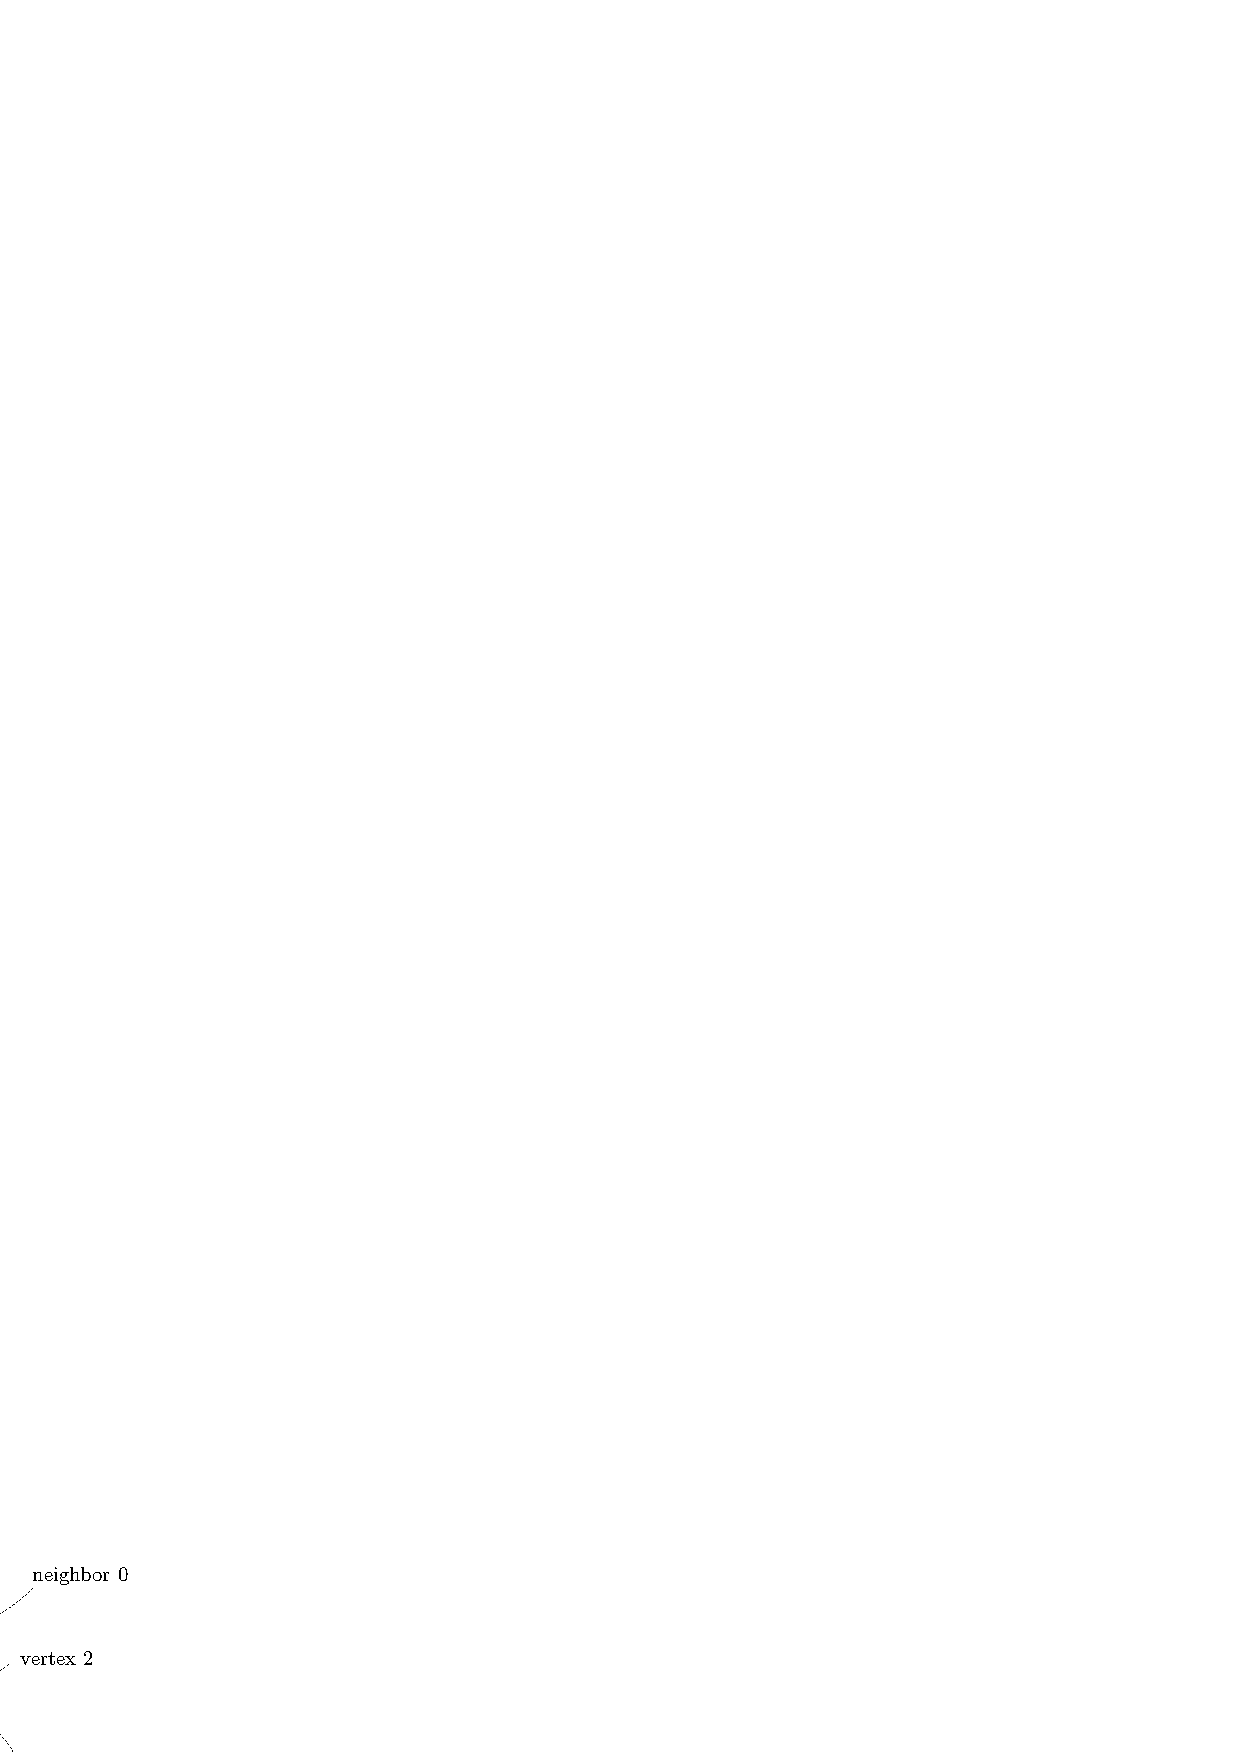
\includegraphics{TriangulationDS_3/repres}
\end{center}
\end{ccTexOnly}
\begin{ccHtmlOnly}
<CENTER>
<img border=0 src="./repres.gif" align=middle alt="Representation">
</CENTER>
\end{ccHtmlOnly}
\caption{Representation.
\label{TDS3-fig-repres}}
\end{figure} 

Edges ($1$-faces) and facets ($2$-faces) are not explicitly
represented: a facet is given by a cell and an index (the facet
\ccc{i} of a cell \ccc{c} is the facet of \ccc{c} that is opposite to
the vertex of index \ccc{i}) and an edge is given by a cell and two
indices (the edge \ccc{(i,j)} of a cell \ccc{c} is the edge
whose endpoints are the vertices of indices \ccc{i} and \ccc{j} of
\ccc{c}). 

\paragraph{Degenerate Dimensions}
As \cgal\ explicitly deals with all degenerate cases, a
3D-triangulation data structure in \cgal\ can handle the cases when
the dimension of the triangulation is lower than~3.

Thus, a 3D-triangulation data structure can store a triangulation of a
topological sphere $S^d$ of $\R^{d+1}$, for any $d \in \{-1,0,1,2,3\}$. 

Let us give, for each dimension, the example corresponding to the
triangulation data structure having a minimal number of vertices, i.e. a 
simplex. These examples are illustrated by presenting their usual
geometric embedding. 
\begin{itemize}
\item \emph{dimension 3.} The triangulation data structure consists of
the boundary of a 4-dimensional simplex, which has 5 vertices. A
geometric embedding consists in choosing one of these vertices to be
infinite, thus four of the five 3-cells become infinite: the geometric
triangulation has one finite tetrahedron remaining, each of its facets
being incident to an infinite cell. See Figure~\ref{TDS3-fig-topo-simplex4}.
\begin{figure}
\begin{ccTexOnly}
\begin{center} 

\includegraphics{TriangulationDS_3/topo-simplex4}
\end{center}
\end{ccTexOnly}
\begin{ccHtmlOnly}
<CENTER>
<img border=0 src="./topo-simplex4.gif" align=middle
alt="4D simplex and a 3D geometric embedding">
</CENTER>
\end{ccHtmlOnly}
\caption{4D simplex and a 3D geometric embedding.
\label{TDS3-fig-topo-simplex4}}
\end{figure} 
\item \emph{dimension 2.} We have 4 vertices forming one 3-dimensional
simplex, i.e. the boundary of a tetrahedron. The geometric embedding in
the plane results from choosing one of these vertices to be infinite,
then the geometric triangulation has one finite triangle whose edges are
incident to the infinite triangles. See Figure~\ref{TDS3-fig-topo-simplex3}.
\begin{figure}
\begin{ccTexOnly}
\begin{center} 
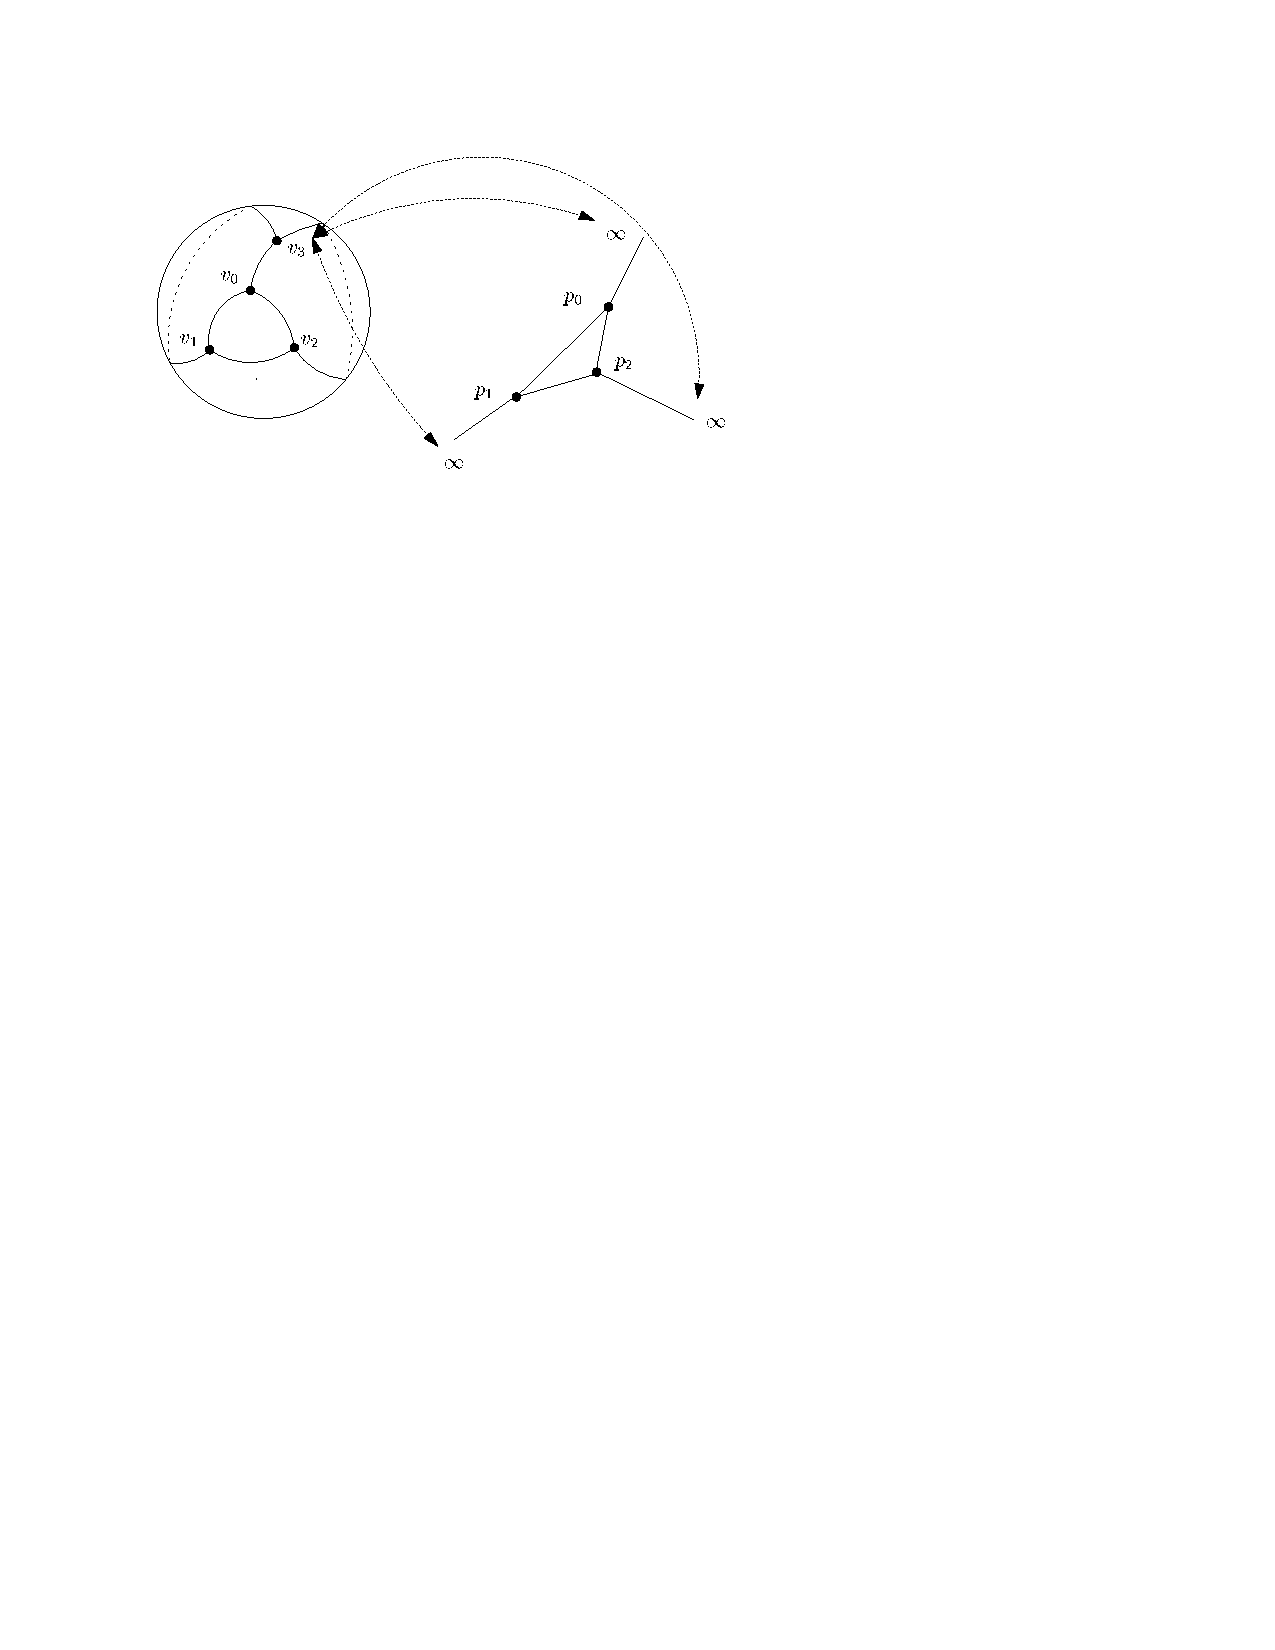
\includegraphics{TriangulationDS_3/topo-simplex3}
\end{center}
\end{ccTexOnly}
\begin{ccHtmlOnly}
<CENTER>
<img border=0 src="./topo-simplex3.gif" align=middle
alt="3D simplex and a 2D geometric embedding">
</CENTER>
\end{ccHtmlOnly}
\caption{3D simplex and a 2D geometric embedding.
\label{TDS3-fig-topo-simplex3}}
\end{figure} 
\item \emph{dimension 1.} A 2-dimensional simplex (a triangle) has 3
vertices. The geometric embedding is an edge whose vertices are linked
to an infinite point.  See Figure~\ref{TDS3-fig-topo-simplex2}.
\begin{figure}
\begin{ccTexOnly}
\begin{center} 
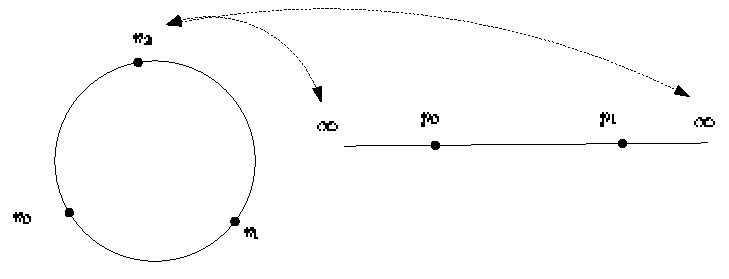
\includegraphics{TriangulationDS_3/topo-simplex2}
\end{center}
\end{ccTexOnly}
\begin{ccHtmlOnly}
<CENTER>
<img border=0 src="./topo-simplex2.gif" align=middle
alt="2D simplex and a 1D geometric embedding">
</CENTER>
\end{ccHtmlOnly}
\caption{2D simplex and a 1D geometric embedding.
\label{TDS3-fig-topo-simplex2}}
\end{figure} 
\end{itemize}

The last three cases are defined uniquely:
\begin{itemize}
\item \emph{dimension 0.} A 0-dimensional triangulation is
combinatorially equivalent to the boundary of a 1-dimensional simplex
(an edge), which consists of 2 vertices. One of them becomes infinite
in the geometric embedding, and there is only one finite vertex
remaining. The two vertices are adjacent.
\item \emph{dimension -1.} This dimension is a convention to represent a 
0-dimensional simplex, that is a sole vertex, which will be
geometrically embedded as an ``empty'' triangulation, having only one
infinite vertex.
\item \emph{dimension -2.} This is also a convention. The
triangulation data structure has no vertex. There is no associated
geometric triangulation.
\end{itemize} 

Note that the notion of infinite vertex has no meaning for the
triangulation data structure. The infinite vertex of the geometric
embedding is a vertex that cannot be distinguished from the other
vertices in the combinatorial triangulation.

The same cell class is used in all cases: triangular faces in
2D can be considered as degenerate cells, having only three vertices
(resp. neighbors) numbered $(0,1,2)$;
edges in 1D have only two vertices (resp. neighbors) numbered $0$ and $1$.

The implicit representation of facets (resp. edges) still holds
for degenerate ($< 3$) dimensions : in dimension~2, each cell has only one
facet of index 3, and 3 edges $(0,1)$, $(1,2)$ and $(2,0)$; in
dimension~1, each cell has one edge $(0,1)$. 

\paragraph{Validity}
A 3D combinatorial triangulation is said to be \ccc{locally valid} 
iff the following is true:

{\bf (a)} When a cell $c$ has a neighbor pointer to another cell $c'$,
then reciprocally this cell $c'$ has a neighbor pointer to $c$, and
$c$ and $c'$ have three vertices in common. These cells are called
adjacent. 
% Two adjacent cells have reciprocal neighbor pointers to each
% other and they have three vertices in common. 

{\bf (b)} The cells have a coherent orientation: if two cells $c_1$
and $c_2$ are adjacent and share a facet with vertices $u,v,w$, then
the vertices of $c_1$ are numbered $(v_0^1 = u, v_1^1 = v, v_2^1 = w,
v_3^1)$, and the vertices of $c_2$ are numbered $(v_0^2 = v, v_1^2 = u,
v_2^2 = w, v_3^2)$, up to positive permutations of $(0,1,2,3)$. In
other words, if we embed the triangulation in $\R^3$, then the fourth
vertices $v_3^1$ and $v_3^2$ of $c_1$ and $c_2$ see the common facet
in opposite orientations. See Figure~\ref{TDS3-fig-comborient}.

The set {\Large $\sigma$}$_4$ of permutations of
$(0,1,2,3)$ has cardinality 24, and the set of positive permutations
$A_4$ has cardinality 12. Thus, for a given orientation, there
are up to 12 different orderings of the four vertices of a cell. Note
that cyclic permutations are negative and so do not preserve the
orientation of a cell.

\begin{figure}[htbp]
\begin{ccTexOnly}
\begin{center} 
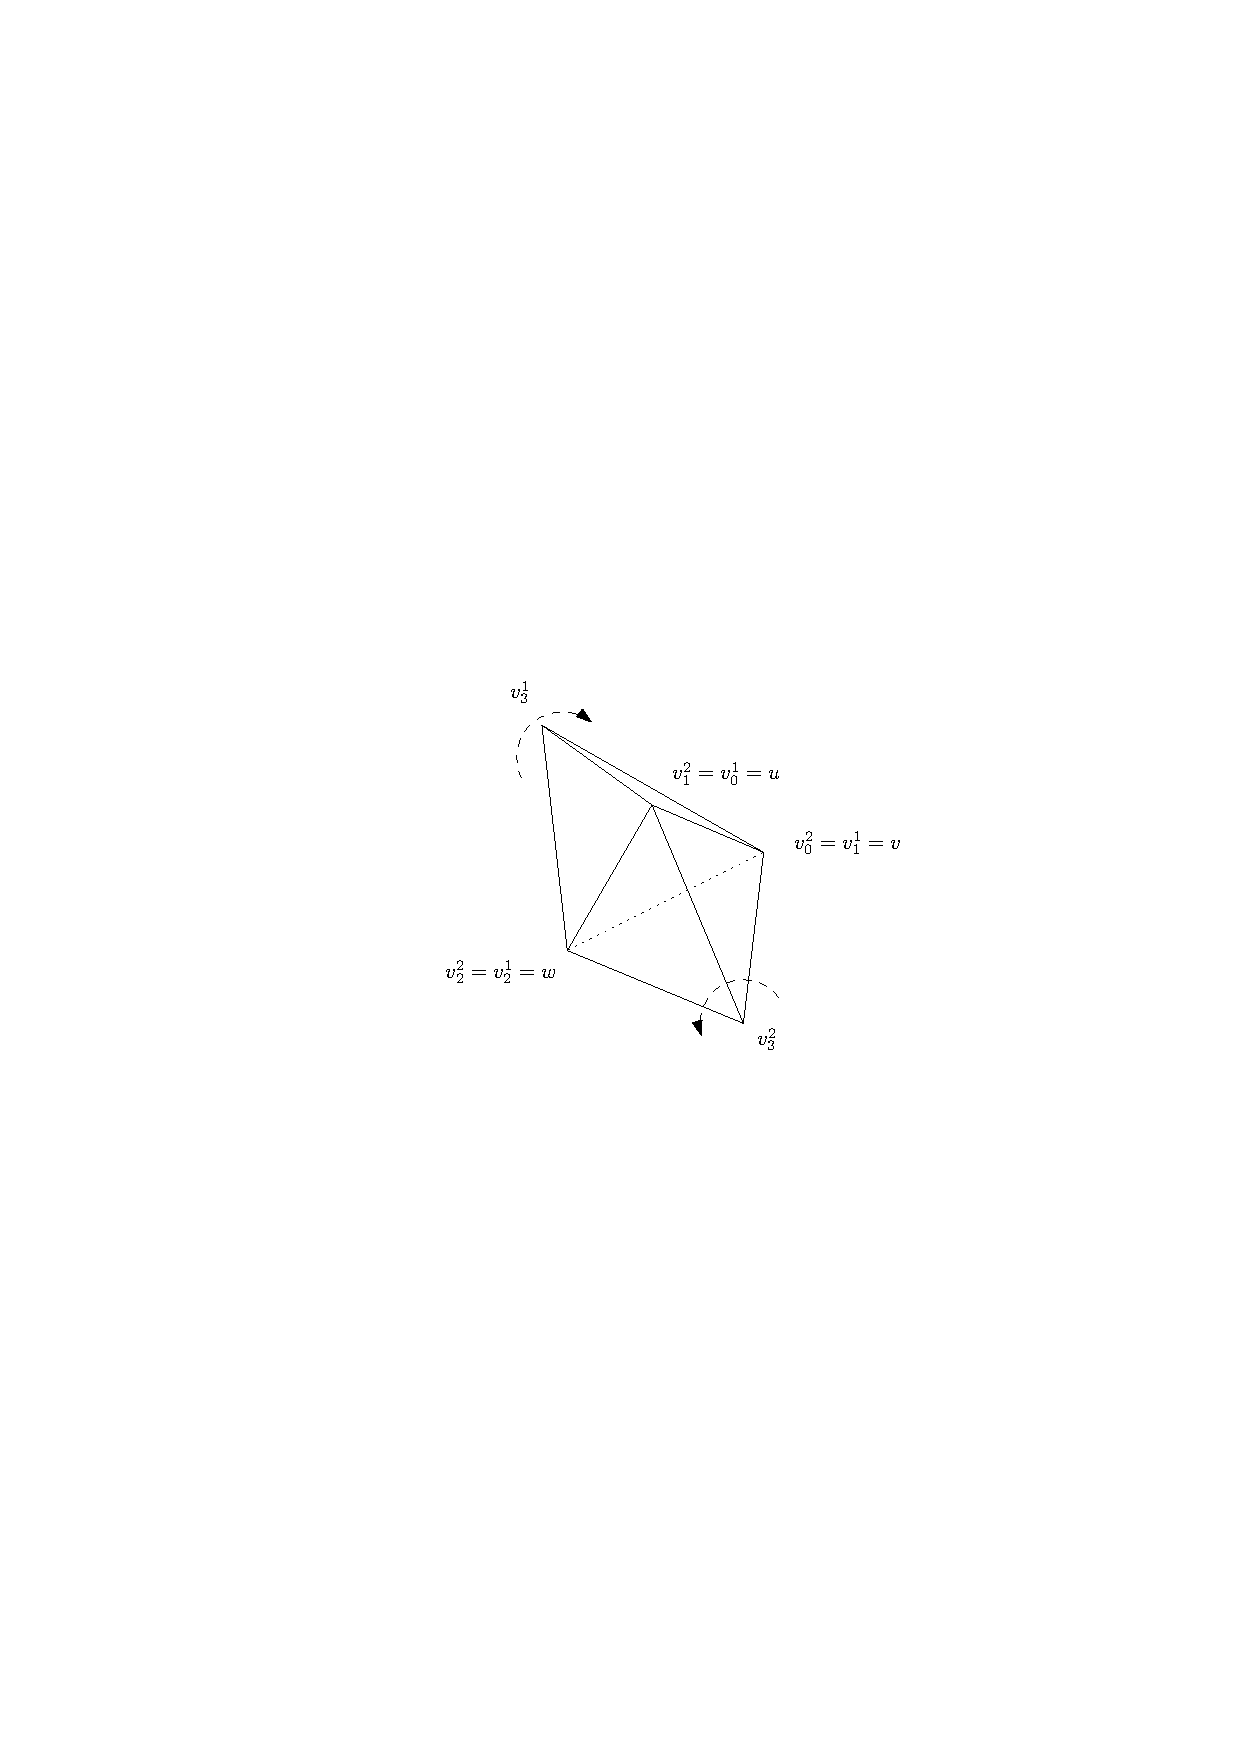
\includegraphics{TriangulationDS_3/comborient} 
\end{center}
\end{ccTexOnly}
\begin{ccHtmlOnly}
<CENTER>
<img border=0 src="./comborient.gif" align=middle alt="Orientation of a cell (3-dimensional case)">
</CENTER>
\end{ccHtmlOnly}
\caption{Coherent orientations of two cells (3-dimensional case).
\label{TDS3-fig-comborient}}
\end{figure} 

The \ccc{is_valid()} method provided by
\ccc{Triangulation_data_structure_3} checks the local validity of a
given triangulation data structure.
 
\section{Software Design\label{TDS3-sec-design}}

The 3D-triangulation data structure class of CGAL,
\ccc{Triangulation_data_structure_3}, is designed to be used as a combinatorial
layer upon which a geometric layer can be built \cite{k-ddsps-98}. This
geometric layer is typically one of the 3D-triangulation classes of \cgal:
\ccc{Triangulation_3}, \ccc{Delaunay_triangulation_3} and
\ccc{Regular_triangulation_3}. This relation is described in more details in
Chapter~\ref{chapter-Triangulation3}, where the
Section~\ref{Triangulation3-sec-design} explains other important parts of the
design related to the geometry.

We focus here on the design of the triangulation data structure (TDS)
itself, which the Figure~\ref{TDS3-fig-layers} illustrates.

\begin{figure}[htbp]
\begin{ccTexOnly}
\begin{center}
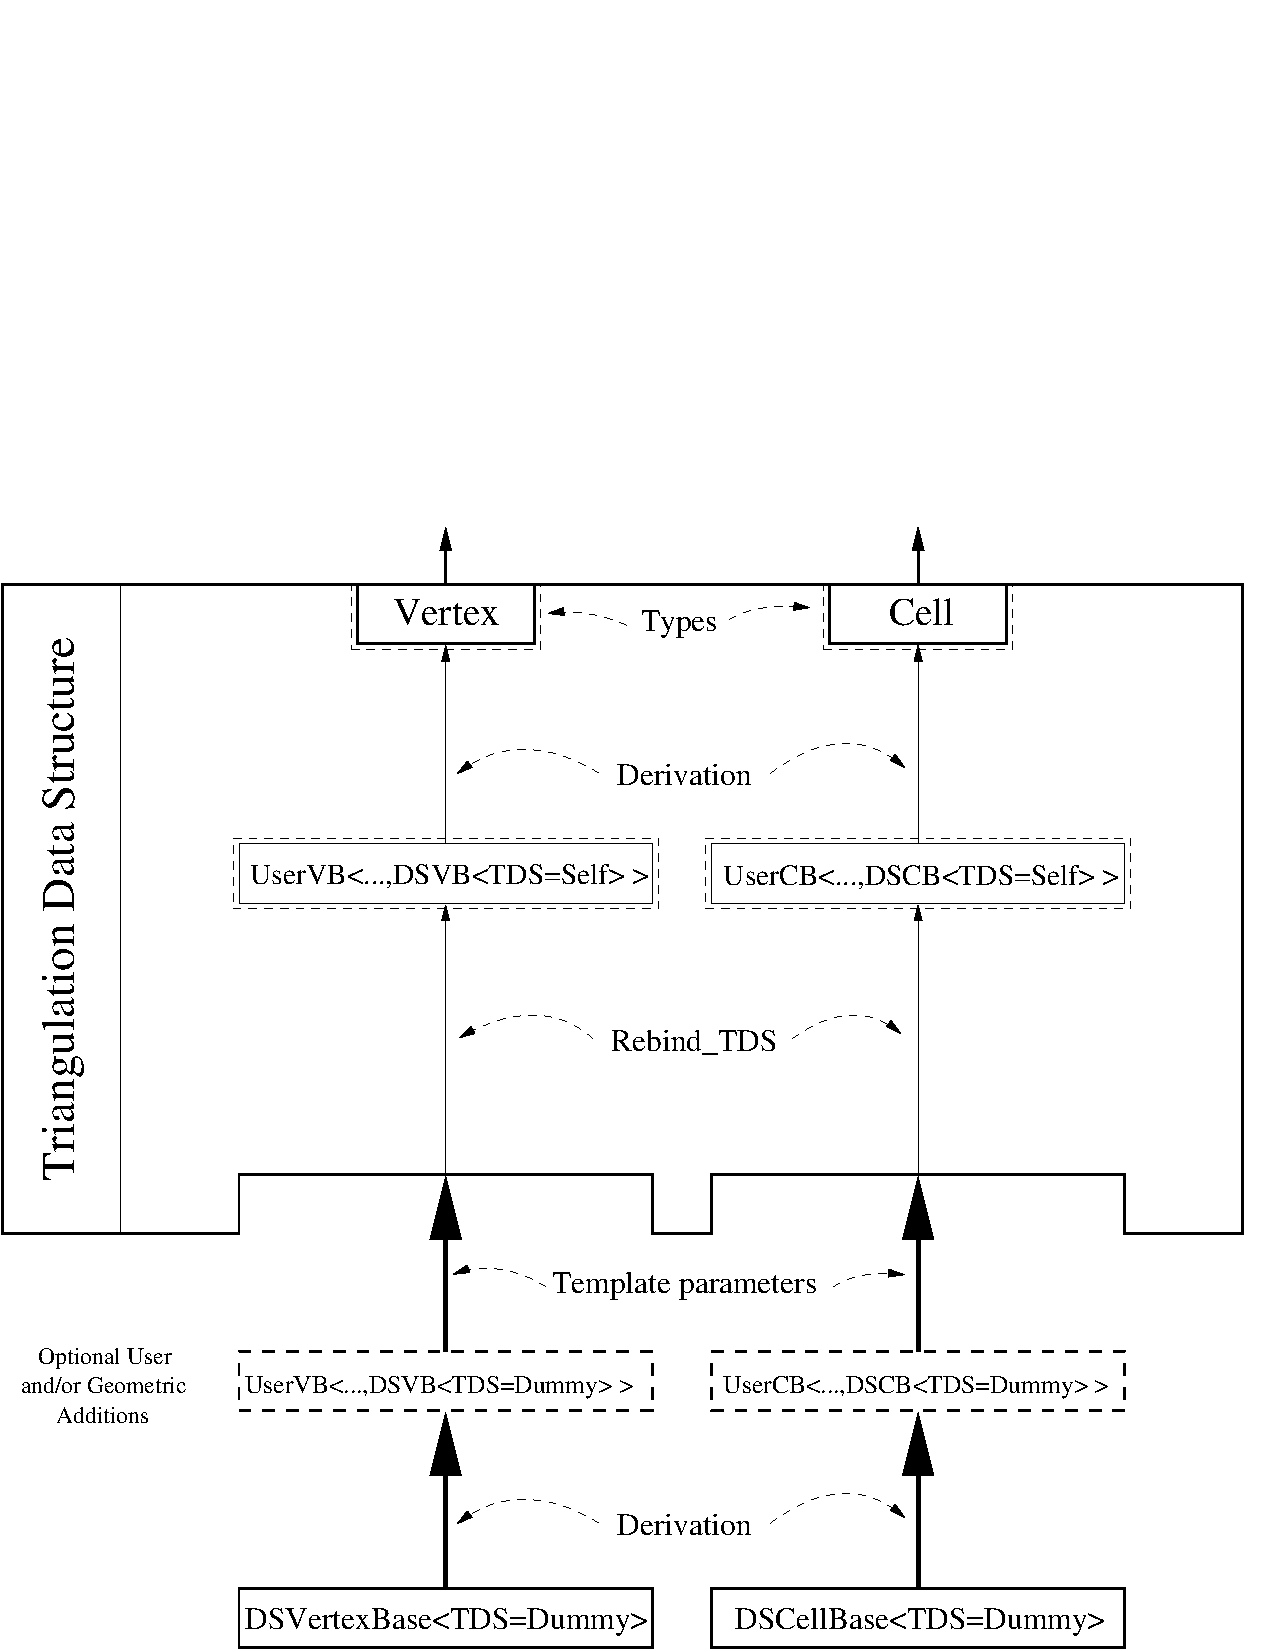
\includegraphics[width=14cm]{TriangulationDS_3/design_tds}
\end{center}
\end{ccTexOnly}
\begin{ccHtmlOnly}
<CENTER>
<img border=0 src="./design_tds.gif" align=middle
 alt="Triangulation Data Structure software design">
</CENTER>
\end{ccHtmlOnly}
\caption{Triangulation Data Structure software design.
\label{TDS3-fig-layers}}
\end{figure} 

\subsection{Flexibility of the Design}

In order for the user to be able to add his own data in the vertices and cells,
the design of the TDS is split into two layers:

\begin{itemize}
\item{} In the bottom layer, the (vertex and cell) base classes store
elementary incidence and adjacency (and possibly geometric or other)
information.  These classes are parameterized by the TDS which provides the
handle types.  (They can also be parameterized by a geometric traits class or
anything else.) A vertex stores a \ccc{Cell_handle}, and a cell stores four
\ccc{Vertex_handle}s and four \ccc{Cell_handle}s.

\item{} The middle layer is the TDS, which is purely combinatorial.  It
provides operations such as insertion of a new vertex in a given cell, on a $1$
or $2$-face. It also allows one, if the dimension of the triangulation is
smaller than $3$, to insert a vertex so that the dimension of the triangulation
is increased by one. The TDS is responsible for the combinatorial integrity of
the eventual geometric triangulation built on top of it (the upper layer,
see Chapter~\ref{chapter-Triangulation3}).
\end{itemize}

The user has several ways to add his own data in the vertex and cell base classes used by the TDS.  He can either:
\begin{itemize}
\item{} use the classes \ccc{Triangulation_vertex_base_with_info}
and \ccc{Triangulation_cell_base_with_info}, which allow to add one data member
of a user provided type, and give access to it.
\item{} derive his own classes from the default base classes
\ccc{Triangulation_ds_vertex_base}, and \ccc{Triangulation_ds_cell_base} (or
the geometric versions typically used by the geometric layer,
\ccc{Triangulation_vertex_base}, and \ccc{Triangulation_cell_base}).
\item{} write his own base classes following the requirements given by the
concepts \ccc{TriangulationCellBase_3} and \ccc{TriangulationVertexBase_3}
\lcTex{(described in \ccRefPage{TriangulationCellBase_3} and
\ccRefPage{TriangulationVertexBase_3})}.
\end{itemize}

\subsection{Cyclic Dependency\label{tds3-cyclic}}

Since adjacency relations are stored in the vertices and cells, it means that
the vertex and cell base classes have to be able to store handles (an entity
akin to pointers) to their neighbors in the TDS.  This in turns means that the
vertex and cell base classes have to know the types of these handles, which are
provided by the TDS.  So in a sense, the base classes are parameterized by the
TDS, and the TDS is parameterized by the vertex and cell base classes !
This is a cycle which cannot be resolved easily.

The solution that we have chosen is similar to the mechanism used by the
standard class \ccc{std::allocator}: the vertex and cell base classes are
initially given a fake or dummy TDS template parameter, whose unique purpose
is to provide the types that can be used by the vertex and cell base classes
(such as handles).  Then, inside the TDS itself, these base classes are
\textit{rebound} to the real TDS type, that is we obtain the same vertex
and cell base classes, but parameterized with the real TDS instead of the dummy
one.  Rebinding is performed by a nested template class of the vertex and cell
base classes (see code below), which provides a type which is the rebound
vertex or cell base class\footnote{It is logically equivalent to a mechanism
that does not exist yet in the C++ language: \textit{template typedef} or
\textit{template aliasing}}.

Here is how it works, schematically:

\begin{ccExampleCode}
template < class Vb, class Cb >
class TDS
{
  typedef TDS<Vb, Cb>    Self;

  // Rebind the vertex and cell base to the actual TDS (Self).
  typedef typename Vb::template Rebind_TDS<Self>::Other  VertexBase;
  typedef typename Cb::template Rebind_TDS<Self>::Other  CellBase;

  // ... further internal machinery leads to the final public types:
public:
  typedef ...  Vertex;
  typedef ...  Cell;
  typedef ...  Vertex_handle;
  typedef ...  Cell_handle;
};

template < class TDS = ... >  // The default is some internal type faking a TDS
class Triangulation_ds_vertex_base_3
{
public:
  template < class TDS2 >
  struct Rebind_TDS {
    typedef Triangulation_ds_vertex_base_3<TDS2>    Other;
  };
...
};
\end{ccExampleCode}

When derivation is used for the vertex or cell base classes, which is the
case at the geometric level with \ccc{Triangulation_vertex_base_3}, then
it gets slightly more involved because its base class has to be rebound as
well:

\begin{ccExampleCode}
template < class GT, class Vb = Triangulation_ds_vertex_base_3<> >
class Triangulation_vertex_base_3 : public Vb
{
public:
  template < class TDS2 >
  struct Rebind_TDS {
    typedef typename Vb::template Rebind_TDS<TDS2>::Other  Vb2;
    typedef Triangulation_vertex_base_3<GT, Vb2>           Other;
  };
...
};
\end{ccExampleCode}

\subsection{Backward Compatibility}
The rebinding scheme has been introduced in CGAL version 3.0.  It is
incompatible with the previous versions, for the cases where the user provides
his own vertex or cell base class.  In these cases, the user needs to add
the rebind nested template class appropriately.  More information is given
in~\ref{T3-sec-compat}.

\section{Examples\label{TDS3-sec-examples}}

\subsection{Incremental construction}
The following example shows how to construct a 3D triangulation data
structure by inserting vertices.

\ccIncludeExampleCode{Triangulation_3/tds.cpp}

\subsection{Cross-linking between a 2D and a 3D data structures}
This example program illustrates how to setup a 2D and a 3D triangulation data
structures whose vertices respectively store vertex handles of the other one.

\ccIncludeExampleCode{Triangulation_3/linking_2d_and_3d.cpp}

%%%%%%%%%%%%%%%%%%%%%%%%%%%%%%%%
\section{Design and Implementation History}

Monique Teillaud introduced the triangulation of the topological
sphere $S^d$ in $\R^{d+1}$ to manage the underlying graph of geometric
triangulations and handle degenerate dimensions \cite{t-tdtc-99}. 

Sylvain Pion improved the software in several ways, in particular
regarding the memory management.

%\end{document}

%%%%%%%%%%%%%%%%%%%%%%%%%%%%%%%%%%%%%%%%%%%%%%%%%%%%%%%%%%%%%%%%%%%%%%%

\usepackage{alltt}           % convinient for programs + a bit of formatting
\usepackage{cc_manual}       % the style what all is about here
\usepackage{cc_manual_index} % the style file for indexing the manual
\usepackage{latex_converter} % the LaTeX to HTML converter style file
\usepackage{amssymb}         % some more math symbols, needed for \mathbb
\usepackage{path}            % for URL's (WWW addresses)
\usepackage{graphicx}        % for PostScript figures
\usepackage{ipe}             % for IPE figures
\usepackage{makeidx}         % for the index
\usepackage{minitoc}         % for the minitable of contents

% page dimensions, for example as used for the CGAL manuals
% ---------------------------------------------------------
\textwidth 15.6cm 
\textheight 23 cm
\topmargin -14mm       
\evensidemargin 3mm 
\oddsidemargin 3mm
\sloppy

\makeindex                   % so the indexing commands have some effect

% New manual style including tab markers on the side margins
% ----------------------------------------------------------
\marginparsep12mm
\marginparwidth13mm
\gdef\ccNewRefManualStyle{\ccTrue}  % undef this for old style manual

% The tab marker are aligned with the top of the main text. To align
% them with the page header, the following redefinition of the actual

% formatting command can be used.
\renewcommand{\ccDrawRefTabs}[2]{%
    \marginpar{~\\\raisebox{12.5mm}[48mm]{%
        \includegraphics{eps_tabs/cc_#1.eps}}}%
}

% Optionally, package authors and a package release can be shown
% right below the chapter title. Comment out the following lines
% to get back to the default behavior.
% -----------------------------------------------------------------
\def\ccTagChapterAuthor{\ccTrue}
\def\ccTagChapterRelease{\ccTrue}

% The colunm layout can be set for all reference pages. Since
% local changes are possible, it is a good idea to enforce the
% the global layout before each reference page. This way, local
% changes of the layout do not change pages in the remainder
% of the manual.
% ------------------------------------------------------------
\newcommand{\cgalColumnLayout}{% example setting of the CGAL manuals
    \ccSetThreeColumns{CGAL_Oriented_side}{}{\hspace*{8.5cm}}%
    \ccPropagateThreeToTwoColumns
}
\cgalColumnLayout

\def\ccRefPageBegin{\ccParDims\cgalColumnLayout}
\def\ccRefPageEnd{\ccParDims\cgalColumnLayout}

% We define the global scope here, for example, to be 'CGAL::'.
% -------------------------------------------------------------
\ccDefGlobalScope{CGAL::}

\begin{document}
% =============================================================================
% The CGAL Reference Manual
% Chapter: Optimisation
% -----------------------------------------------------------------------------
% file  : doc_tex/basic/Optimisation/main.tex
% author: Bernd G�rtner, Sven Sch�nherr (sven@inf.fu-berlin.de)
% -----------------------------------------------------------------------------
% $Revision$
% $Date$
% =============================================================================

\newcommand{\linebreakByHand}{\ccTexHtml{\\}{}}
\newcommand{\SaveSpaceByHand}{}  %%%% [2]{\ccTexHtml{#1}{#2}}

\chapter{Geometric Optimisation} \label{Optimisation}
\RCSdefDate{\OptRCSDate}{$Date$}

\ccChapterRelease{Release: 2.0 \ccTexHtml{\quad}{ , } \OptRCSDate}

\ccChapterAuthor{Bernd G{\"a}rtner}\ccTexHtml{\\}{<br>}
\ccChapterAuthor{Michael Hoffmann}\ccTexHtml{\\}{<br>}
\ccChapterAuthor{Sven Sch{\"o}nherr}

\ccTexHtml{\thispagestyle{empty}}{}

\begin{ccTexOnly}\section*{Introduction}\end{ccTexOnly}
\begin{ccHtmlOnly}<H2>Introduction</H2><P>\end{ccHtmlOnly}

This chapter describes routines for solving geometric optimisation problems.
The first two sections contain algorithms for computing and updating the
smallest enclosing circle (Section~\ref{sec:smallest_enclosing_circles})
resp.\ ellipse (Section~\ref{sec:smallest_enclosing_ellipses}) of a finite
point set.  Formally, the `smallest enclosing circle' is the boundary of the
closed disk of minimum area covering the point set. It is known that this
disk is unique.  We usually identify the disk with its bounding circle,
allowing us to talk about points being on the boundary of the circle, etc.
The same holds for the smallest enclosing ellipse. These algorithms work in
an incremental manner. They are implemented as semi-dynamic data structures,
thus allowing to insert points while maintaining the smallest enclosing
circle resp.\ ellipse.

The remaining sections describe algorithms for searching in matrices with
specific properties and some applications. In particular, there are
general implementations of
\begin{itemize}
  \item monotone matrix search (see Section~\ref{secMonotoneMatrixSearch}),
    which can be applied to compute
    \begin{itemize}
      \item extremal polygons of a convex polygon
        (see Section~\ref{secComputingExtremalPolygons}) \textit{or}
      \item all furthest neighbors for the vertices of a convex polygon
        (see Section~\ref{secAllFurthestNeighbors}),
    \end{itemize}
  \item and sorted matrix search (see Section~\ref{secSortedMatrixSearch}),
    which can be used to compute the $p$-centers of a planar point set
    (see Section~\ref{sec_RectangularPCenters}).
\end{itemize}

\subsubsection*{Traits Class}
The class and function templates are parameterized with a traits class
which defines the abstract interface between the optimisation
algorithm and the primitives it uses. We provide traits class
implementations that interface the optimisation algorithms with the
\cgal\ kernel. For some algorithms, in addition, we provide traits
class adapters to user supplied point classes. Finally, we describe
the requirements that must be fulfilled by traits classes for
optimisation algorithms.  This is at the same time a specification for
using the provided traits class implementations as for users who want
to supply their own traits class.

\subsubsection*{Assertions}
The optimisation code uses infix \ccc{OPTIMISATION} in the assertions,
e.g.\ defining the compiler flag
\ccc{CGAL_OPTIMISATION_NO_PRECONDITIONS} switches precondition
checking off, cf.~Section~\ref{assertions}.

\newcommand{\cgalSetOptTraitsAdaptLayout}{\ccTexHtml{%
    \ccSetThreeColumns{CGAL_Oriented_side}{}{returns constants
      \ccc{CGAL_LEFTTURN}, \ccc{CGAL_COLLINEAR}}
    \ccPropagateThreeToTwoColumns}{}}
\newcommand{\cgalSetOptTraitsAdaptReqLayout}{\ccTexHtml{%
    \ccSetThreeColumns{CGAL_Oriented_side}{da.get_hw( Point p).}{}
    \ccPropagateThreeToTwoColumns}{}}

\newcommand{\cgalSetOptTraitsReqLayout}{\ccTexHtml{%
    \ccSetThreeColumns{CGAL_Oriented_side}{}{returns
      \ccc{CGAL_ON_BOUNDED_SIDE}, \ccc{CGAL_ON_BOUNDARY}}
    \ccPropagateThreeToTwoColumns}{}}

\ccHtmlNoClassToc

\input{smallest_enclosing_circles}

\input{smallest_enclosing_ellipses}

%% ==============================================================
%% Specification: Computing Extremal Polygons
%% --------------------------------------------------------------
%% file  : spec_extremal_polygons.awi
%% author: Michael Hoffmann
%% $Id$
%% ==============================================================

\clearpage
\section{Computing Extremal Polygons}
\label{secComputingExtremalPolygons}
\cgalColumnLayout

This section describes several functions to compute a maximal $k$-gon
$P_k$ that can be inscribed into a given convex polygon $P$. The
criterion for maximality can be chosen freely by defining an
appropriate traits class as specified in section
\ref{req_ExtremalPolygonTraits}. For \cgal\ point classes there are
two predefined traits classes to compute a maximum area (see section
\ref{secMaximumAreaInscribedKgon}) resp.  perimeter (see section
\ref{secMaximumPerimeterInscribedKgon}) inscribed $k$-gon.

\ccHtmlNoClassToc
\begin{ccHtmlClassFile}{computing_maximum_area_inscribed_k_gon.html}
  {Function Declaration of \ccc{maximum_area_inscribed_k_gon}}
  \ccHtmlNoClassIndex\ccHtmlNoClassLinks
  %% class wrapper to keep the font at a uniform size:
  \begin{ccClass}{dummy}
    \ccHtmlNoIndex\subsection{Computing a Maximum Area Inscribed $k$-gon}
  \label{secMaximumAreaInscribedKgon}
  \end{ccClass}
  
  This section describes a function to compute a maximal area $k$-gon
  $P_k$ that can be inscribed into a given convex polygon $P$. Note
  that $P_k$ is not unique in general, but it can be chosen in such a
  way that its vertices form a subset of the vertex set of $P$.

  \ccInclude{CGAL/extremal_polygon_2.h}

  \def\ccLongParamLayout{\ccTrue} 
  
  \ccGlobalFunction{
    template < class RandomAccessIC, class OutputIterator >
    OutputIterator
    maximum_area_inscribed_k_gon(
    RandomAccessIC points_begin,
    RandomAccessIC points_end,
    int k,
    OutputIterator o);}
  
  computes a maximum area inscribed $k$-gon of the convex polygon
  described by [\ccc{points_begin}, \ccc{points_end}), writes its
  vertices to \ccc{o} and returns the past-the-end iterator of this
  sequence.
  
  \ccHeading{Precondition}
  \begin{enumerate}
  \item Value type of \ccc{RandomAccessIC} has to be
    \ccc{Point_2<R>} for some representation class \ccc{R}.
  \item \ccc{OutputIterator} accepts the value type of
    \ccc{RandomAccessIC} as value type,
  \item the -- at least three -- points denoted by the range
    [\ccc{points_begin}, \ccc{points_end}) form the boundary of a convex
    polygon (oriented clock-- or counterclockwise) \textit{and}
  \item $k \ge 3$.
  \end{enumerate}

  \ccHeading{Note}
  
  On compilers not supporting member function templates, the parameter
  \ccc{RandomAccessIC} is fixed to \ccc{vector<Point_2>::iterator}
  where \ccc{Point_2} is the value type of \ccc{RandomAccessIC}.
  
  \ccImplementation The implementation uses monotone matrix
  search\cite{akmsw-gamsa-87} and has a worst case running time of $O(k
  \cdot n + n \cdot \log n)$, where $n$ is the number of vertices in
  $P$.

  \ccExample The following code generates a random convex polygon
  \ccc{p} with ten vertices and computes the maximum area inscribed
  five-gon of \ccc{p}.

  \ccIncludeVerbatim{extremal_polygon_2_example_area.C}

\end{ccHtmlClassFile}
    
\ccHtmlNoClassToc
\begin{ccHtmlClassFile}{computing_maximum_perimeter_inscribed_k_gon.html}
  {Function Declaration of \ccc{maximum_perimeter_inscribed_k_gon}}
  \ccHtmlNoClassIndex\ccHtmlNoClassLinks
  %% class wrapper to keep the font at a uniform size:
  \begin{ccClass}{dummy}
    \ccHtmlNoIndex\subsection{Computing a Maximum Perimeter Inscribed
      $k$-gon}
    \label{secMaximumPerimeterInscribedKgon}
  \end{ccClass}
  
  This section describes a function to compute a largest perimeter
  $k$-gon $P_k$ that can be inscribed in a given convex polygon $P$.
  Note that $P_k$ is not unique in general, but we know that its
  vertices form a subset of the vertex set of $P$.

  \ccInclude{CGAL/extremal_polygon_2.h}

  \def\ccLongParamLayout{\ccTrue}
  \ccGlobalFunction{
    template < class RandomAccessIC, class OutputIterator >
    OutputIterator
    maximum_perimeter_inscribed_k_gon(
    RandomAccessIC points_begin,
    RandomAccessIC points_end,
    int k,
    OutputIterator o);}
  
  computes a maximum perimeter inscribed $k$-gon of the convex polygon
  described by [\ccc{points_begin}, \ccc{points_end}), writes its
  vertices to \ccc{o} and returns the past-the-end iterator of this
  sequence.

  \ccHeading{Precondition}
  \begin{enumerate}
  \item Value type of \ccc{RandomAccessIC} has to be
    \ccc{Point_2<R>} for some representation class \ccc{R},
  \item there is a global function \ccc{R::FT sqrt( R::FT)}
    defined that computes the squareroot of a number,
  \item \ccc{OutputIterator} accepts the value type of
    \ccc{RandomAccessIC} as value type,
  \item the -- at least three -- points denoted by the range
    [\ccc{points_begin}, \ccc{points_end}) form the boundary of a
    convex polygon (oriented clock-- or counterclockwise) \textit{and}
  \item $k \ge 2$.
  \end{enumerate}

  \ccTagDefaults

  \ccHeading{Note}
  
  On compilers not supporting member function templates, the parameter
  \ccc{RandomAccessIC} is fixed to \ccc{vector<Point_2>::iterator}
  where \ccc{Point_2} is the value type of \ccc{RandomAccessIC}.
  
  \ccImplementation The implementation uses monotone matrix
  search\cite{akmsw-gamsa-87} and has a worst case running time of $O(k
  \cdot n + n \cdot \log n)$, where $n$ is the number of vertices in
  $P$.

  \ccExample The following code generates a random convex polygon
  \ccc{p} with ten vertices and computes the maximum perimeter inscribed
  five-gon of \ccc{p}.

  \ccIncludeVerbatim{extremal_polygon_2_example_perimeter.C}

\end{ccHtmlClassFile}

\begin{ccAdvanced}
  \ccHtmlNoClassToc
  \begin{ccHtmlClassFile}{computing_general_extremal_polygons.html}
    {Function Declaration of \ccc{extremal_polygon}}
    \ccHtmlNoClassIndex\ccHtmlNoClassLinks
    %% class wrapper to keep the font at a uniform size:
    \begin{ccClass}{dummy}
      \ccHtmlNoIndex\subsection{Computing General Extremal
        Polygons}\label{secGeneralExtremalPolygons}
    \end{ccClass}
    
    This section describes a general function to compute a maximal
    $k$-gon $P_k$ that can be inscribed in a given convex polygon $P$.
    The criterion for maximality and some basic operations have to
    specified in an appropriate traits class as specified in section
    \ref{req_ExtremalPolygonTraits}.
    
    \ccInclude{CGAL/extremal_polygons_2.h}

    \def\ccLongParamLayout{\ccTrue} 
    
    \ccGlobalFunction{
      template < class RandomAccessIC, class OutputIterator, class Traits >
      OutputIterator
      extremal_polygon(
      RandomAccessIC points_begin,
      RandomAccessIC points_end,
      int k,
      OutputIterator o,
      const Traits& t);}
    
    computes a maximal (as specified by \ccc{t}) inscribed $k$-gon of
    the convex polygon described by [\ccc{points_begin},
    \ccc{points_end}), writes its vertices to \ccc{o} and returns the
    past-the-end iterator of this sequence.
    
    \ccHeading{Precondition}
    \begin{enumerate}
    \item \ccc{Traits} has to satisfy the requirements stated in section
      \ref{req_ExtremalPolygonTraits},
    \item Value type of \ccc{RandomAccessIC} must be
      \ccc{Traits::Point_2},
    \item \ccc{OutputIterator} accepts \ccc{Traits::Point_2} as value
      type,
    \item the -- at least three -- points denoted by the range
      [\ccc{points_begin}, \ccc{points_end}) form the boundary of a
      convex polygon (oriented clock-- or counterclockwise) \textit{and}
    \item $k \ge \ccc{t.min_k()}$.
    \end{enumerate}
    
    \ccImplementation The implementation uses monotone matrix
    search\cite{akmsw-gamsa-87} and has a worst case running time of
    $O(k \cdot n + n \cdot \log n)$, where $n$ is the number of vertices
    in $P$.
  \end{ccHtmlClassFile}
  
  \ccHtmlNoClassToc\ccHtmlNoClassIndex\begin{ccClass}{Exp_traits}
    \ccCreationVariable{t}\ccTagFullDeclarations
    
    \subsection{Requirements for Extremal Polygon Traits
      Classes}\label{req_ExtremalPolygonTraits}
    
    \ccDefinition A class \ccClassName\ has to provide the following
    types and operations in order to qualify as a traits class for
    \ccc{extremal_polygon}.
    
    \ccTypes 
    
    \ccNestedType{Point_2}{class used for representing the input
      points.}
    
    \ccNestedType{FT}{class used for doing computations on point
      coordinates (has to fulfill field-type requirements).}
    
    \ccNestedType{Operation}{AdaptableBinaryFunction class \ccc{op}:
      \ccc{Point_2} $\times$ \ccc{Point_2} $\rightarrow$ \ccc{FT}.
      Together with \ccc{init} this operation recursively defines the
      objective function to maximize.  Let $p$ and $q$ be two vertices
      of a polygon $P$ such that $q$ precedes $p$ in the oriented
      vertex chain of $P$ starting with vertex $root$.  Then
      \ccc{op(p,q)} returns the value by which an arbitrary
      sub-polygon of $P$ with vertices from $[root,\, q]$ increases
      when $p$ is added to it. E.g. in the maximum area case this is
      the area of the triangle $(root,\, q,\, p)$.}

    \ccOperations
    
    \ccMemberFunction{int min_k() const;}{returns the minimal $k$ for
      which a maximal $k$-gon can be computed. (e.g. in the maximum
      area case this is three.)}
    
    \ccMemberFunction{FT init( const Point_2& p, const Point_2& q)
      const;}{returns the value of the objective function for a
      polygon consisting of the two points \ccc{p} and \ccc{q}. (e.g.
      in the maximum area case this is \ccc{FT( 0)}.)}
    
    \ccMemberFunction{Operation operation( const Point_2& p)
      const;}{return \ccc{Operation} where \ccc{p} is the fixed $root$
      point.}
    
    \ccMemberFunction{template < class RandomAccessIC, class
      OutputIterator > OutputIterator compute_min_k_gon(
      RandomAccessIC points_begin, RandomAccessIC points_end, FT&
      max_area, OutputIterator o) const;}{writes the points of
      [\ccc{points_begin}, \ccc{points_end}) forming a
      \ccc{min_k()}-gon rooted at \ccc{points_begin[0]} of maximal
      value to o and returns the past-the-end iterator for that
      sequence (== \ccc{o + min_k()}).}
    
    \ccMemberFunction{template < class RandomAccessIC > bool
      is_convex( RandomAccessIC points_begin, RandomAccessIC
      points_end) const;}{returns true, iff the points
      [\ccc{points_begin}, \ccc{points_end}) form a convex chain.}
    
    \ccHeading{Notes}
    \begin{itemize}
    \item \ccClassName\ccc{::is_convex} is only used for precondition
      checking. Therefore it needs not to be specified, in case that
      precondition checking is disabled.
    \item On compilers not supporting member function templates,
      \ccc{RandomAccessIC} is fixed to \ccc{vector<Point_2>::iterator}
      and \ccc{OutputIterator} is fixed to
      \ccc{vector<int>::reverse_iterator}.
      
    \end{itemize}
    
    \ccSeeAlso \ccInclude{CGAL/Extremal_polygon_traits_2.h}
    
    The classes \ccc{Kgon_area_traits<R>} and
    \ccc{Kgon_perimeter_traits<R>} (templatized with a \cgal\ 
    representation class) both fulfill these requirements.
    
  \end{ccClass}
\end{ccAdvanced}

%% --------------------------------------------------------------
%% EOF spec_extremal_polygons.awi
%% --------------------------------------------------------------

 
%% ==============================================================
%% Specification: All Furthest Neighbors
%% --------------------------------------------------------------
%% file  : spec_all_furthest_neighbors.awi
%% author: Michael Hoffmann
%% $Id$
%% ==============================================================

\cgalColumnLayout

\begin{ccRefFunction}{all_furthest_neighbors_2}
  
  \ccDefinition The function \ccRefName\ computes all furthest
  neighbors for the vertices of a convex polygon $P$, i.e. for each
  vertex $v$ of $P$ a vertex $f_v$ of $P$ such that the distance
  between $v$ and $f_v$ is maximized.

  \ccInclude{CGAL/all_furthest_neighbors_2.h}

  \def\ccLongParamLayout{\ccTrue} 
  
  \ccGlobalFunction{ template < class RandomAccessIC, class
    OutputIterator, class Traits > OutputIterator
    all_furthest_neighbors_2( RandomAccessIC points_begin,
    RandomAccessIC points_end, OutputIterator o, Traits t =
    Default_traits);}
  
  computes all furthest neighbors for the vertices of the convex
  polygon described by the range [\ccc{points_begin},
  \ccc{points_end}), writes their indices (relative to
  \ccc{points_begin}) to \ccc{o}\footnote{i.e. the furthest neighbor
    of \ccc{points_begin[}i\ccc{]} is \ccc{points_begin[}$i$-th number
    written to \ccc{o}\ccc{]}} and returns the past-the-end iterator
  of this sequence.
  
  \ccPrecond The points denoted by the non-empty range
  [\ccc{points_begin}, \ccc{points_end}) form the boundary of a convex
  polygon $P$ (oriented clock-- or counterclockwise).
  
  The geometric types and operations to be used for the computation
  are specified by the traits class parameter \ccc{t}. This parameter
  can be omitted if \ccc{RandomAccessIC} refers to a point type from
  the 2D-Kernel. In this case, a default traits class
  (\ccc{All_furthest_neighbors_default_traits_2<R>}) is used.
  
  \ccRequire
  \begin{enumerate}
  \item If \ccc{t} is specified explicitly, \ccc{Traits} is a model
    for \ccc{All_furthest_neighbors_traits_2}.
  \item Value type of \ccc{RandomAccessIC} is \ccc{Traits::Point_2} or
    -- if \ccc{t} is not specified explicitly -- \ccc{Point_2<R>} for
    some representation class \ccc{R}.
  \item \ccc{OutputIterator} accepts \ccc{int} as value type.
  \end{enumerate}
  
  \ccSeeAlso
  \ccRefIdfierPage{All_furthest_neighbors_traits_2}\\
  \ccRefIdfierPage{CGAL::All_furthest_neighbors_default_traits_2<R>}\\
  \ccRefIdfierPage{CGAL::monotone_matrix_search}
 
  \ccImplementation The implementation uses monotone matrix
  search\cite{akmsw-gamsa-87}. Its runtime complexity is linear in the
  number of vertices of $P$.
  
  \ccExample The following code generates a random convex polygon
  \ccc{p} with ten vertices, computes all furthest neighbors and
  writes the sequence of their indices (relative to
  \ccc{points_begin}) to \ccc{cout} (e.g. a sequence of
  \ccc{4788911224} means the furthest neighbor of
  \ccc{points_begin[0]} is \ccc{points_begin[4]}, the furthest
  neighbor of \ccc{points_begin[1]} is \ccc{points_begin[7]} etc.).
  
  \ccIncludeVerbatim{Optimisation_ref/all_furthest_neighbors_2_example_noheader.C}
\end{ccRefFunction}

\begin{ccRefClass}{All_furthest_neighbors_default_traits_2<R>}
  \ccCreationVariable{t}\ccTagFullDeclarations
  
  \ccDefinition The class \ccClassName\ provides the types and
  operations needed to compute all furthest neighbors for the vertices
  of a convex polygon.
  
  \ccRequirements
  The template parameter \ccc{R} is a model for \ccc{Kernel}.

  \ccIsModel 
  \ccRefIdfierPage{All_furthest_neighbors_traits_2}

  \ccTypes
  
  \ccNestedType{Point_2}{typedef to \ccc{R::Point_2}.}
  
  \ccNestedType{FT}{typedef to \ccc{R::FT}.}
  
  \ccNestedType{Distance}{AdaptableBinaryFunction class: \ccc{Point_2}
    $\times$ \ccc{Point_2} $\rightarrow$ \ccc{FT} computing the
    squared Euclidean distance between two points.}

  \ccOperations
  
  \ccMemberFunction{Distance distance_object();}{returns the
    function object for computing distances.}
  
  \ccMemberFunction{template < class RandomAccessIC > bool is_convex(
    RandomAccessIC points_begin, RandomAccessIC points_end)
    const;}{returns true, iff the points [\ccc{points_begin},
    \ccc{points_end}) form a convex chain.}
  
  \ccSeeAlso
  \ccRefIdfierPage{CGAL::all_furthest_neighbors_2}

  \ccHeading{Notes}
  \begin{itemize}
  \item \ccClassName\ccc{::is_convex} is used for precondition
    checking only.
  \end{itemize}
\end{ccRefClass}

\begin{ccRefConcept}{All_furthest_neighbors_traits_2}
  \ccCreationVariable{t}\ccTagFullDeclarations
  
  \ccDefinition The concept \ccRefName\ defines types and operations
  needed to compute all furthest neighbors for the vertices of a
  convex polygon using the function \ccc{all_furthest_neighbors_2}.
  
  \ccTypes
  
  \ccNestedType{Point_2}{class used for representing the input
    points.}
  
  \ccNestedType{FT}{class used for doing computations on point
    coordinates; it has to be a model for \ccc{FieldNumberType}.}
  
  \ccNestedType{Distance}{AdaptableBinaryFunction class: \ccc{Point_2}
    $\times$ \ccc{Point_2} $\rightarrow$ \ccc{FT} computing the
    squared Euclidean distance between two points.}

  \ccOperations
  
  \ccMemberFunction{Distance distance_object();}{returns the
    function object for computing distances.}
  
  \ccMemberFunction{template < class RandomAccessIC > bool is_convex(
    RandomAccessIC points_begin, RandomAccessIC points_end)
    const;}{returns true, iff the points [\ccc{points_begin},
    \ccc{points_end}) form a convex chain.}
  
  \ccHasModels 
  \ccRefIdfierPage{CGAL::All_furthest_neighbors_default_traits_2<R>}

  \ccSeeAlso
  \ccRefIdfierPage{CGAL::all_furthest_neighbors_2}

  \ccHeading{Notes}
  \begin{itemize}
  \item \ccClassName\ccc{::is_convex} is used for precondition
    checking only.
  \end{itemize}
\end{ccRefConcept}

%% --------------------------------------------------------------
%% EOF spec_all_furthest_neighbors.awi
%% --------------------------------------------------------------

 
%% ==============================================================
%% Specification: Rectangular p-Centers
%% --------------------------------------------------------------
%% file  : spec_rectangular_p_centers.awi
%% author: Michael Hoffmann
%% $Id$
%% ==============================================================

\cgalColumnLayout

\begin{ccRefFunction}{rectangular_p_center_2}
  \ccIndexMainItem[t]{rectilinear centers}
  \ccIndexMainItem[t]{rectangular centers}
  \ccIndexSubitem[t]{center}{rectangular}
  
  \ccDefinition The function \ccRefName\ computes rectilinear
  $p$-centers of a planar point set, i.e. a set of $p$ points such
  that the maximum minimal $L_{\infty}$-distance between both sets is
  minimized.
  
  More formally the problem can be defined as follows.
  
  \ccTexHtml{Given a finite set $\mathcal{P}$ of points, compute a
    point set $\mathcal{C}$ with $|\mathcal{C}| \le p$ such that the
    $p$-radius of $\mathcal{P}$,
    $$
    rad_p(\mathcal{P}) := \max_{P \in \mathcal{P}} \min_{Q \in
      \mathcal{C}} || P - Q ||_\infty
    $$
    is minimized. We can interpret $\mathcal{C}$ as the best
    approximation (with respect to the given metric) for $\mathcal{P}$
    with at most $p$ points.}{Given a finite set <IMG WIDTH=12
    HEIGHT=12 ALIGN=BOTTOM ALT="tex2html_wrap_inline17"
    SRC="./MatrixSearch_pcenter1.gif" > of points, compute a point set
    <IMG WIDTH=9 HEIGHT=13 ALIGN=BOTTOM ALT="tex2html_wrap_inline19"
    SRC="./MatrixSearch_pcenter2.gif" > with <IMG WIDTH=46 HEIGHT=24
    ALIGN=MIDDLE ALT="tex2html_wrap_inline21"
    SRC="./MatrixSearch_pcenter3.gif" > such that the <I>p</I>-radius
    of <IMG WIDTH=12 HEIGHT=12 ALIGN=BOTTOM
    ALT="tex2html_wrap_inline17" SRC="./MatrixSearch_pcenter1.gif" > ,
    <P> <IMG WIDTH=358 HEIGHT=24 ALIGN=BOTTOM ALT="displaymath27"
    SRC="./MatrixSearch_pcenter4.gif" > <P> is minimized. We can
    interpret <IMG WIDTH=9 HEIGHT=13 ALIGN=BOTTOM
    ALT="tex2html_wrap_inline19" SRC="./MatrixSearch_pcenter2.gif" >
    as the best approximation (with respect to the given metric) for
    <IMG WIDTH=12 HEIGHT=12 ALIGN=BOTTOM ALT="tex2html_wrap_inline17"
    SRC="./MatrixSearch_pcenter1.gif" > with at most <I>p</I> points.}

  \ccInclude{CGAL/rectangular_p_center_2.h}

  \def\ccLongParamLayout{\ccTrue} 
  
  \ccGlobalFunction{template < class ForwardIterator, class
    OutputIterator, class FT, class Traits > OutputIterator
    rectangular_p_center_2(ForwardIterator f, ForwardIterator l,
    OutputIterator o, FT& r, int p, const Traits& t =
    Default_traits);}
  
  computes rectilinear \ccc{p}-centers for the point set described by
  the range [\ccc{f}, \ccc{l}), sets \ccc{r} to the corresponding
  $p$-radius, writes the at most \ccc{p} center points to \ccc{o} and
  returns the past-the-end iterator of this sequence.
  
  \ccPrecond
  \begin{enumerate}
  \item The range [\ccc{f}, \ccc{l}) is not empty.
  \item 2 $\le$ \ccc{p} $\le$ 4.
  \end{enumerate}
  
  The geometric types and operations to be used for the computation
  are specified by the traits class parameter \ccc{t}. This parameter
  can be omitted if \ccc{ForwardIterator} refers to a point type from
  the 2D-Kernel. In this case, a default traits class
  (\ccc{Rectangular_p_center_default_traits_2<R>}) is used.
  
  \ccRequire
  \begin{enumerate}
  \item \textit{Either: (if no traits parameter is given)} Value type
    of \ccc{ForwardIterator} is \ccc{CGAL::Point_2<R>} for some
    representation class \ccc{R} and \ccc{FT} is equivalent to
    \ccc{R::FT},
  \item \textit{Or: (if a traits parameter is specified)} \ccc{Traits}
    is a model for \ccc{RectangularPCenterTraits_2}.
  \item \ccc{OutputIterator} accepts the value type of
    \ccc{ForwardIterator} as value type.
  \end{enumerate}  
  
  \ccSeeAlso
  \ccRefConceptPage{RectangularPCenterTraits_2}\\
  \ccRefIdfierPage{CGAL::Rectangular_p_center_default_traits_2<R>}\\
  \ccRefIdfierPage{CGAL::sorted_matrix_search}
  
  \ccImplementation The runtime is linear for $p \in \{2,\,3\}$ and
  $\mathcal{O}(n \cdot \log n)$ for $p = 4$ where $n$ is the number of
  input points. These runtimes are worst case optimal. The $3$-center
  algorithm uses a prune-and-search technique described in
  \cite{cgal:h-slacr-99}.  The $4$-center implementation uses sorted matrix
  search \cite{fj-fkppc-83,fj-gsrsm-84} and fast algorithms for
  piercing rectangles \cite{sw-rpppp-96}.
  
  \ccExample The following code generates a random set of ten points
  and computes its two-centers.

  \ccIncludeExampleCode{Matrix_search/rectangular_p_center_2_example_nohead.cpp}
\end{ccRefFunction}

\begin{ccRefClass}{Rectangular_p_center_default_traits_2<R>}
  \ccCreationVariable{t}\ccTagFullDeclarations
    
  \ccDefinition The class \ccRefName\ defines types and operations
  needed to compute rectilinear $p$-centers of a planar point set
  using the function \ccc{rectangular_p_center_2}.
  
  \ccRequirements The template parameter \ccc{R} is a model for
  \ccc{Kernel}.
  
  \ccIsModel
  \ccRefConceptPage{RectangularPCenterTraits_2}

  \ccTypes 
    
  \ccNestedType{FT}{typedef to \ccc{R::FT}.}
  
  \ccNestedType{Point_2}{typedef to \ccc{R::Point_2}.}
  
  \ccNestedType{Iso_rectangle_2}{typedef to \ccc{R::Iso_rectangle_2}.}
  
  \ccNestedType{Less_x_2}{typedef to \ccc{R::Less_x_2}.}
 
  \ccNestedType{Less_y_2}{typedef to \ccc{R::Less_y_2}.}
  
  \ccNestedType{Construct_vertex_2}{typedef to
    \ccc{R::Construct_vertex_2}.}
  
  \ccNestedType{Construct_iso_rectangle_2}{typedef to
    \ccc{R::Construct_iso_rectangle_2}.}
    
  \ccNestedType{Signed_x_distance_2}{adaptable binary function
    class: \ccc{Point_2} $\times$ \ccc{Point_2} $\rightarrow$
    \ccc{FT} returns the signed distance of two points'
    $x$-coordinates.}
  
  \ccNestedType{Signed_y_distance_2}{adaptable binary function
    class: \ccc{Point_2} $\times$ \ccc{Point_2} $\rightarrow$
    \ccc{FT} returns the signed distance of two points'
    $y$-coordinates.}
  
  \ccNestedType{Infinity_distance_2}{adaptable binary function
    class: \ccc{Point_2} $\times$ \ccc{Point_2} $\rightarrow$
    \ccc{FT} returns the $||\cdot||_{\infty}$ distance of two
    points.}
  
  \ccNestedType{Signed_infinity_distance_2}{adaptable binary
    function class: \ccc{Point_2} $\times$ \ccc{Point_2}
    $\rightarrow$ \ccc{FT} returns the signed $||\cdot||_{\infty}$
    distance of two points.}
  
  \ccNestedType{Construct_point_2_below_left_implicit_point_2}{
    3-argument function class: \ccc{Point_2} $\times$ \ccc{Point_2}
    $\times$ \ccc{FT} $\rightarrow$ \ccc{Point_2}. For arguments
    $(p,\,q,\,r)$ it returns the lower-left corner of the iso-oriented
    square with sidelength $r$ and upper-right corner at the
    intersection of the vertical line through $p$ and the horizontal
    line through $q$.}
    
  \ccNestedType{Construct_point_2_below_right_implicit_point_2}{
    3-argument function class: \ccc{Point_2} $\times$ \ccc{Point_2}
    $\times$ \ccc{FT} $\rightarrow$ \ccc{Point_2}. For arguments
    $(p,\,q,\,r)$ it returns the lower-right corner of the
    iso-oriented square with sidelength $r$ and upper-left corner at
    the intersection of the vertical line through $p$ and the
    horizontal line through $q$.}
    
  \ccNestedType{Construct_point_2_above_right_implicit_point_2}{
    3-argument function class: \ccc{Point_2} $\times$ \ccc{Point_2}
    $\times$ \ccc{FT} $\rightarrow$ \ccc{Point_2}. For arguments
    $(p,\,q,\,r)$ it returns the upper-right corner of the
    iso-oriented square with sidelength $r$ and lower-left corner at
    the intersection of the vertical line through $p$ and the
    horizontal line through $q$.}
    
  \ccNestedType{Construct_point_2_above_left_implicit_point_2}{
    3-argument function class: \ccc{Point_2} $\times$ \ccc{Point_2}
    $\times$ \ccc{FT} $\rightarrow$ \ccc{Point_2}. For arguments
    $(p,\,q,\,r)$ it returns the upper-left corner of the iso-oriented
    square with sidelength $r$ and lower-right corner at the
    intersection of the vertical line through $p$ and the horizontal
    line through $q$.}

  \ccOperations
  
  For every function class listed above there is a member function
  to fetch the corresponding function object.
  
  \ccMemberFunction{Inf_distance_2 inf_distance_2_object() const;}{}
  \ccGlue\ccMemberFunction{Signed_inf_distance_2
    signed_inf_distance_2_object() const;}{}
  
  \ccGlue\ccMemberFunction{Construct_vertex_2
    construct_vertex_2_object() const;}{}
  
  \ccGlue\ccMemberFunction{Construct_iso_rectangle_2
    construct_iso_rectangle_2_object() const;}{}
  
  \ccGlue\ccMemberFunction{Construct_iso_rectangle_2_below_left_point_2
    construct_iso_rectangle_2_below_left_point_2_object() const;}{}
  
  \ccGlue\ccMemberFunction{Construct_iso_rectangle_2_above_left_point_2
    construct_iso_rectangle_2_above_left_point_2_object() const;}{}
  
  \ccGlue\ccMemberFunction{Construct_iso_rectangle_2_below_right_point_2
    construct_iso_rectangle_2_below_right_point_2_object() const;}{}
  
  \ccGlue\ccMemberFunction{Construct_iso_rectangle_2_above_right_point_2
    construct_iso_rectangle_2_above_right_point_2_object() const;}{}
  
  \ccSeeAlso
  \ccRefIdfierPage{CGAL::rectangular_p_center_2}

\end{ccRefClass}

\begin{ccRefConcept}{RectangularPCenterTraits_2}
  \ccCreationVariable{t}\ccTagFullDeclarations
    
  \ccDefinition The concept \ccRefName\ defines types and operations
  needed to compute rectilinear $p$-centers of a planar point set
  using the function \ccc{rectangular_p_center_2}.
  
  \ccTypes 
    
  \ccNestedType{FT}{model for \ccRefConceptPage{FieldNumberType}.}
  
  \ccNestedType{Point_2}{model for
    \ccRefConceptPage{Kernel::Point_2}.}
  
  \ccNestedType{Iso_rectangle_2}{model for
    \ccRefConceptPage{Kernel::Iso_rectangle_2}.}
  
  \ccNestedType{Less_x_2}{model for
    \ccRefConceptPage{Kernel::Less_x_2}.}
  
  \ccNestedType{Less_y_2}{model for
    \ccRefConceptPage{Kernel::Less_y_2}.}
  
  \ccNestedType{Construct_vertex_2}{model for
    \ccRefConceptPage{Kernel::Construct_vertex_2}.}
  
  \ccNestedType{Construct_iso_rectangle_2}{model for
    \ccRefConceptPage{Kernel::Construct_iso_rectangle_2}.}
    
  \ccNestedType{Signed_x_distance_2}{adaptable binary function
    class: \ccc{Point_2} $\times$ \ccc{Point_2} $\rightarrow$
    \ccc{FT} returns the signed distance of two points'
    $x$-coordinates.}
  
  \ccNestedType{Signed_y_distance_2}{adaptable binary function
    class: \ccc{Point_2} $\times$ \ccc{Point_2} $\rightarrow$
    \ccc{FT} returns the signed distance of two points'
    $y$-coordinates.}
  
  \ccNestedType{Infinity_distance_2}{adaptable binary function
    class: \ccc{Point_2} $\times$ \ccc{Point_2} $\rightarrow$
    \ccc{FT} returns the $||\cdot||_{\infty}$ distance of two
    points.}
  
  \ccNestedType{Signed_infinity_distance_2}{adaptable binary
    function class: \ccc{Point_2} $\times$ \ccc{Point_2}
    $\rightarrow$ \ccc{FT} returns the signed $||\cdot||_{\infty}$
    distance of two points.}
  
  \ccNestedType{Construct_point_2_below_left_implicit_point_2}{
    3-argument function class: \ccc{Point_2} $\times$ \ccc{Point_2}
    $\times$ \ccc{FT} $\rightarrow$ \ccc{Point_2}. For arguments
    $(p,\,q,\,r)$ it returns the lower-left corner of the iso-oriented
    square with sidelength $r$ and upper-right corner at the
    intersection of the vertical line through $p$ and the horizontal
    line through $q$.}
    
  \ccNestedType{Construct_point_2_below_right_implicit_point_2}{
    3-argument function class: \ccc{Point_2} $\times$ \ccc{Point_2}
    $\times$ \ccc{FT} $\rightarrow$ \ccc{Point_2}. For arguments
    $(p,\,q,\,r)$ it returns the lower-right corner of the
    iso-oriented square with sidelength $r$ and upper-left corner at
    the intersection of the vertical line through $p$ and the
    horizontal line through $q$.}
    
  \ccNestedType{Construct_point_2_above_right_implicit_point_2}{
    3-argument function class: \ccc{Point_2} $\times$ \ccc{Point_2}
    $\times$ \ccc{FT} $\rightarrow$ \ccc{Point_2}. For arguments
    $(p,\,q,\,r)$ it returns the upper-right corner of the
    iso-oriented square with sidelength $r$ and lower-left corner at
    the intersection of the vertical line through $p$ and the
    horizontal line through $q$.}
    
  \ccNestedType{Construct_point_2_above_left_implicit_point_2}{
    3-argument function class: \ccc{Point_2} $\times$ \ccc{Point_2}
    $\times$ \ccc{FT} $\rightarrow$ \ccc{Point_2}. For arguments
    $(p,\,q,\,r)$ it returns the upper-left corner of the iso-oriented
    square with sidelength $r$ and lower-right corner at the
    intersection of the vertical line through $p$ and the horizontal
    line through $q$.}

  \ccOperations
  
  For every function class listed above there is a member function
  to fetch the corresponding function object.
  
  \ccMemberFunction{Inf_distance_2 inf_distance_2_object() const;}{}
  \ccGlue\ccMemberFunction{Signed_inf_distance_2
    signed_inf_distance_2_object() const;}{}
  
  \ccGlue\ccMemberFunction{Construct_vertex_2
    construct_vertex_2_object() const;}{}
  
  \ccGlue\ccMemberFunction{Construct_iso_rectangle_2
    construct_iso_rectangle_2_object() const;}{}
  
  \ccGlue\ccMemberFunction{Construct_iso_rectangle_2_below_left_point_2
    construct_iso_rectangle_2_below_left_point_2_object() const;}{}
  
  \ccGlue\ccMemberFunction{Construct_iso_rectangle_2_above_left_point_2
    construct_iso_rectangle_2_above_left_point_2_object() const;}{}
  
  \ccGlue\ccMemberFunction{Construct_iso_rectangle_2_below_right_point_2
    construct_iso_rectangle_2_below_right_point_2_object() const;}{}
  
  \ccGlue\ccMemberFunction{Construct_iso_rectangle_2_above_right_point_2
    construct_iso_rectangle_2_above_right_point_2_object() const;}{}
  
  \ccHasModels
  \ccRefIdfierPage{CGAL::Rectangular_p_center_default_traits_2<R>}

  \ccSeeAlso
  \ccRefIdfierPage{CGAL::rectangular_p_center_2}

\end{ccRefConcept}

%% --------------------------------------------------------------
%% EOF spec_rectangular_p_centers.awi
%% --------------------------------------------------------------

 
%% ==============================================================
%% Specification: Monotone Matrix Search
%% --------------------------------------------------------------
%% file  : spec_monotone_matrix_search.awi
%% author: Michael Hoffmann
%% $Id$
%% ==============================================================

\cgalColumnLayout

\begin{ccRefFunction}{monotone_matrix_search}
  \begin{ccAdvanced}
    
    \ccDefinition The function \ccRefName\ computes the maxima for all
    rows of a totally monotone matrix.
    
    More precisely, monotony for matrices is defined as follows.
    
    \ccTexHtml{Let $K$ be a totally ordered set, $M \in K^{(n,\, m)}$
      a matrix over $K$ and for $0 \le i < n$:
      $$
      rmax_M(i) :\in \left\{ \min_{0 \le j < m} j \: \left|\:
          M[i,\, j] = \max_{0 \le k < m} M[i,\, k] \right.\right\}
      $$
      the (leftmost) column containing the maximum entry in row
      $i$.  $M$ is called monotone, iff
      $$
      \forall\, 0 \le i_1 < i_2 < n\: :\: rmax_M(i_1) \le
      rmax_M(i_2)\; .
      $$
      $M$ is totally monotone, iff all of its submatrices are
      monotone (or equivalently: iff all $2 \times 2$ submatrices are
      monotone).}{Let <I>K</I> be a totally ordered set, <IMG WIDTH=84
      HEIGHT=31 ALIGN=MIDDLE ALT="tex2html_wrap_inline11"
      SRC="./MatrixSearch_totmon1.gif" > a matrix over <I>K</I> and
      for <IMG WIDTH=64 HEIGHT=24 ALIGN=MIDDLE
      ALT="tex2html_wrap_inline13" SRC="./MatrixSearch_totmon2.gif" >
      : <P> <IMG WIDTH=427 HEIGHT=39 ALIGN=BOTTOM ALT="displaymath15"
      SRC="./MatrixSearch_totmon3.gif" > <P> the (leftmost) column
      containing the maximum entry in row <I>i</I>.  <I>M</I> is
      called monotone, iff <P> <IMG WIDTH=411 HEIGHT=16 ALIGN=BOTTOM
      ALT="displaymath19" SRC="./MatrixSearch_totmon4.gif" > <P>
      <I>M</I> is totally monotone, iff all of its submatrices are
      monotone (or equivalently: iff all <IMG WIDTH=33 HEIGHT=20
      ALIGN=MIDDLE ALT="tex2html_wrap_inline21"
      SRC="./MatrixSearch_totmon5.gif" > submatrices are monotone).}
    
    \ccInclude{CGAL/monotone_matrix_search.h}

    \def\ccLongParamLayout{\ccTrue} 
    \ccTexHtml{%
      \ccSetThreeColumns{void}{}{\hspace*{8.5cm}}
      \ccPropagateThreeToTwoColumns}{}
    
    \ccGlobalFunction{template < class Matrix, class RandomAccessIC,
      class Compare_strictly > void monotone_matrix_search( const
      Matrix& m, RandomAccessIC t, const Compare_strictly&
      compare_strictly = less< Matrix::Value >());}
    
    computes the maximum (as specified by \ccc{compare_strictly})
    entry for each row of \ccc{m} and writes the corresponding column
    to \ccc{t}, i.e. \ccc{t[i]} is set to the index of the column
    containing the maximum element in row \ccc{i}. The maximum $m_r$
    of a row $r$ is the leftmost element for which
    \ccc{compare_strictly}$(m_r,\,x)$ is false for all elements $x$ in
    $r$.
    
    \cgalColumnLayout
    \ccPrecond \ccc{t} points to a structure of size at least
    \ccc{m.number_of_rows()}

    \ccRequire
    \begin{enumerate}
    \item \ccc{Matrix} is a model for
      \ccc{Monotone_matrix_search_traits}.
    \item Value type of \ccc{RandomAccessIC} is \ccc{int}.
    \item If \ccc{compare_strictly} is defined, it is an adaptable
      binary function: \ccc{Matrix::Value} $\times$
      \ccc{Matrix::Value} $\rightarrow$ \ccc{bool} describing a strict
      (non-reflexive) total ordering on \ccc{Matrix::Value}.
    \end{enumerate}
    
    \ccSeeAlso
    \ccRefIdfierPage{Monotone_matrix_search_traits}\\
    \ccRefIdfierPage{\ccPureGlobalScope all_furthest_neighbors_2}\\
    \ccRefIdfierPage{\ccPureGlobalScope maximum_area_inscribed_k_gon_2}\\
    \ccRefIdfierPage{\ccPureGlobalScope maximum_perimeter_inscribed_k_gon_2}\\
    \ccRefIdfierPage{\ccPureGlobalScope extremal_polygon_2}

    \ccImplementation The implementation uses an algorithm by Aggarwal
    et al.\cite{akmsw-gamsa-87}. The runtime is linear in the number
    of rows and columns of the matrix.

  \end{ccAdvanced}  
\end{ccRefFunction}

\begin{ccRefClass}{Dynamic_matrix<M>}
  \begin{ccAdvanced}
    \ccCreationVariable{d}\ccTagDefaults
    
    \ccDefinition The class \ccClassTemplateName\ is an adaptor for an
    arbitrary matrix class \ccc{M} to provide the dynamic operations
    needed for monotone matrix search.
    
    \ccRequirements \ccc{M} is a model for \ccc{Basic_matrix}.
    
    \ccInclude{CGAL/Dynamic_matrix.h}
    
    \ccIsModel
    \ccRefIdfierPage{Monotone_matrix_search_traits}\\
    \ccRefIdfierPage{Basic_matrix}

    \ccCreation
    
    \ccConstructor{Dynamic_matrix( const M& m);}{initializes
      \ccVar\ to \ccc{m}. \ccc{m} is \textit{not} copied, we only
      store a reference.}

    \ccOperations
    
    \ccMemberFunction{int number_of_columns() const;}{returns the
      number of columns.}
    
    \ccMemberFunction{int number_of_rows() const;}{returns the number
      of rows.}
    
    \ccMemberFunction{Entry operator()( int row, int column) const;}
    {returns the entry at position (\ccc{row}, \ccc{column}).
      \ccPrecond\\ $0 \le$ \ccc{row} $<$ \ccc{number_of_rows()} and\\ 
      $0 \le$ \ccc{column} $<$ \ccc{number_of_columns()}.}
    
    \ccMemberFunction{void replace_column( int old, int new);}{replace
      column \ccc{old} with column number \ccc{new}.  \ccPrecond\\ $0
      \le$ \ccc{old}, \ccc{new} $<$ \ccc{number_of_columns()}.}
    
    \ccMemberFunction{Matrix* extract_all_even_rows() const;}{returns
      a new Matrix consisting of all rows of \ccVar\ with even index,
      (i.e. first row is row $0$ of \ccVar, second row is row $2$ of
      \ccVar\ etc.). \ccPrecond \ccc{number_of_rows()} $> 0$.}
    
    \ccMemberFunction{void shrink_to_quadratic_size();}{deletes the
      rightmost columns, such that \ccVar\ becomes quadratic.
      \ccPrecond\\ \ccc{number_of_columns()} $\ge$
      \ccc{number_of_rows()}. \ccPostcond\\ \ccc{number_of_rows()}
      $==$ \ccc{number_of_columns()}.}
    
    \ccSeeAlso
    \ccRefIdfierPage{\ccPureGlobalScope monotone_matrix_search}\\
    \ccRefIdfierPage{Monotone_matrix_search_traits}\\
    \ccRefIdfierPage{Basic_matrix}

    \ccImplementation All operations take constant time except for
    \ccc{extract_all_even_rows} which needs time linear in the number
    of rows.
    
  \end{ccAdvanced}
\end{ccRefClass}

\begin{ccRefConcept}{Monotone_matrix_search_traits}
  \begin{ccAdvanced}
    \ccCreationVariable{m}\ccTagFullDeclarations
    
    \ccDefinition The concept \ccRefName\ is a refinement of
    \ccc{Basic_matrix} and defines types and operations needed to
    compute the maxima for all rows of a totally monotone matrix using
    the function \ccc{monotone_matrix_search}.
    
    \ccTypes
    
    \ccNestedType{Value}{The type of a matrix entry.}

    \ccOperations
    
    \ccMemberFunction{int number_of_columns() const;}{returns the
      number of columns.}
    
    \ccMemberFunction{int number_of_rows() const;}{returns the number
      of rows.}
    
    \ccMemberFunction{Entry operator()( int row, int column) const;}
    {returns the entry at position (\ccc{row}, \ccc{column}).
      \ccPrecond\\ $0 \le$ \ccc{row} $<$ \ccc{number_of_rows()} and\\
      $0 \le$ \ccc{column} $<$ \ccc{number_of_columns()}.}
    
    \ccMemberFunction{void replace_column( int old, int new);}{replace
      column \ccc{old} with column number \ccc{new}.  \ccPrecond\\ $0
      \le$ \ccc{old}, \ccc{new} $<$ \ccc{number_of_columns()}.}
    
    \ccMemberFunction{Matrix* extract_all_even_rows() const;}{returns
      a new Matrix consisting of all rows of \ccVar\ with even index,
      (i.e. first row is row $0$ of \ccVar, second row is row $2$ of
      \ccVar\ etc.). \ccPrecond \ccc{number_of_rows()} $> 0$.}
    
    \ccMemberFunction{void shrink_to_quadratic_size();}{deletes the
      rightmost columns, such that \ccVar\ becomes quadratic.
      \ccPrecond\\ \ccc{number_of_columns()} $\ge$
      \ccc{number_of_rows()}. \ccPostcond\\ \ccc{number_of_rows()} $==$
      \ccc{number_of_columns()}.}
    
    \ccHeading{Notes}
    \begin{itemize}
    \item For the sake of efficiency (and in order to achieve the time
      bounds claimed for \ccc{monotone_matrix_search}), all these
      operations have to be realized in constant time -- except for
      \ccc{extract_all_even_rows} which may take linear time.
    \item There is an adaptor \ccc{Dynamic_matrix} that can be used to
      add most of the functionality described above to arbitrary
      matrix classes.
    \end{itemize}
    
    \ccHasModels
    \ccRefIdfierPage{\ccPureGlobalScope Dynamic_matrix<M>}

    \ccSeeAlso
    \ccRefIdfierPage{\ccPureGlobalScope monotone_matrix_search}

  \end{ccAdvanced}
\end{ccRefConcept}

\begin{ccRefConcept}{Basic_matrix}
  \begin{ccAdvanced}
    \ccCreationVariable{m}\ccTagFullDeclarations
    
    \ccDefinition A class \ccClassName\ has to provide the following
    types and operations in order to be a model for
    \ccc{Basic_matrix}.
    
    \ccTypes
    
    \ccNestedType{Value}{The type of a matrix entry. It has to define
      a copy constructor.}
    
    \ccOperations
    
    \ccMemberFunction{int number_of_columns() const;}{returns the
      number of columns.}
    
    \ccMemberFunction{int number_of_rows() const;}{returns the
      number of rows.}
    
    \ccMemberFunction{Entry operator()( int row, int column) const;}
    {returns the entry at position (\ccc{row}, \ccc{column}).
      \ccPrecond\\ $0 \le$ \ccc{row} $<$ \ccc{number_of_rows()} and\\
      $0 \le$ \ccc{column} $<$ \ccc{number_of_columns()}.}

    \ccHasModels
    \ccRefIdfierPage{\ccPureGlobalScope Dynamic_matrix<M>}

    \ccSeeAlso
    \ccRefIdfierPage{Monotone_matrix_search_traits}\\
    \ccRefIdfierPage{Sorted_matrix_search_traits}
    
  \end{ccAdvanced}
\end{ccRefConcept}

%% --------------------------------------------------------------
%% EOF spec_monotone_matrix_search.awi
%% --------------------------------------------------------------

 
%% ==============================================================
%% Specification: Sorted Matrix Search
%% --------------------------------------------------------------
%% file  : spec_sorted_matrix_search.awi
%% author: Michael Hoffmann
%% $Id$
%% ==============================================================

\cgalColumnLayout
  
\begin{ccRefFunction}{sorted_matrix_search}
  \ccIndexMainItem[t]{sorted matrix search}
  \ccIndexSubitem[t]{searching}{in sorted matrices}
  \ccIndexSubitem[t]{matrix}{sorted}
  \ccIndexSubitem[t]{matrix}{searching}
  \ccIndexMainItem[t]{Frederickson/Johnson matrix search}
  
  \begin{ccAdvanced}
    \ccDefinition The function \ccRefName\ selects the smallest entry
    in a set of sorted matrices that fulfills a certain feasibility
    criterion.
    
    \ccTexHtml{More exactly, a matrix $M = (m_{i j}) \in S^{r \times
        l}$ (over a totally ordered set $S$) is sorted, iff
      \begin{eqnarray*}
        \forall \, 1 \le i \le r,\; 1 \le j < l\; :\; m_{i j} \le m_{i (j+1)} 
        \;\; {\it and}\\ 
        \forall \, 1 \le i < r,\; 1 \le j \le l\; :\; m_{i j} \le m_{(i+1) j} 
        \;\;.
      \end{eqnarray*}
      
      Now let $\mathcal{M}$ be a set of $n$ sorted matrices over $S$
      and $f$ be a monotone predicate on $S$, i.e.
      $$
      f\: :\: S \longrightarrow\, \textit{bool} \quad{\rm with}\quad f(r)
      \;\Longrightarrow\; \forall\, t \in S\,,\: t > r \; :\; f(t)\;.
      $$}{More exactly, a matrix <IMG WIDTH=124 HEIGHT=30 ALIGN=MIDDLE
      ALT="tex2html_wrap_inline18" SRC="./MatrixSearch_sorted1.gif" >
      (over a totally ordered set <I>S</I>) is sorted, iff <P> <IMG
      WIDTH=500 HEIGHT=41 ALIGN=BOTTOM ALT="eqnarray5"
      SRC="./MatrixSearch_sorted2.gif" > <P> <P> Now let <IMG WIDTH=18
      HEIGHT=13 ALIGN=BOTTOM ALT="tex2html_wrap_inline22"
      SRC="./MatrixSearch_sorted3.gif" > be a set of <I>n</I> sorted
      matrices over <I>S</I> and <I>f</I> be a monotone predicate on
      <I>S</I>, i.e.  <P> <IMG WIDTH=445 HEIGHT=16 ALIGN=BOTTOM
      ALT="displaymath32" SRC="./MatrixSearch_sorted4.gif" > <P><BR>}
    
    If we assume there is any feasible element in one of the matrices
    in \ccTexHtml{$\mathcal{M}$}{<IMG WIDTH=18 HEIGHT=13 ALIGN=BOTTOM
      ALT="tex2html_wrap_inline21" SRC="./MatrixSearch_sorted3.gif"
      >}, there certainly is a smallest such element. This is the one
    we are searching for.
    
    The feasibility test as well as some other parameters can (and
    have to) be customized through a traits class. 
    
    \ccInclude{CGAL/sorted_matrix_search.h}

    \def\ccLongParamLayout{\ccTrue} 
    
    \ccGlobalFunction{template < class RandomAccessIC, class Traits >
      Traits::Value sorted_matrix_search( RandomAccessIC f,
      RandomAccessIC l, const Traits& t);}

    returns the element \ccc{x} in one of the sorted matrices from the
    range $\left[ f,\, l \right)$, for which \ccc{t.is_feasible( x)}
    is true and \ccc{t.compare( x, y)} is true for all other
    \ccc{y} values from any matrix for which \ccc{t.is_feasible(
      y)} is true.
    
    \ccPrecond
    \begin{enumerate}
    \item All matrices in $\left[f,\, l\right)$ are sorted according
      to \ccc{Traits::compare_non_strictly}.
    \item There is at least one entry $x$ in a matrix $M \in
      \left[f,\, l\right)$ for which \ccc{Traits::is_feasible(x)} is
      true.
    \end{enumerate}
    
    \ccRequire
    \begin{enumerate}
    \item \ccc{Traits} is a model for
      \ccc{Sorted_matrix_search_traits}.
    \item Value type of \ccc{RandomAccessIC} is \ccc{Traits::Matrix}.
    \end{enumerate}
    
    \ccSeeAlso
    \ccRefConceptPage{Sorted_matrix_search_traits}
    
    \ccImplementation The implementation uses an algorithm by
    Frederickson and Johnson\cite{fj-fkppc-83,fj-gsrsm-84} and runs in
    $\mathcal{O}(n \cdot k + f \cdot \log (n \cdot k))$, where $n$ is
    the number of input matrices, $k$ denotes the maximal dimension of
    any input matrix and $f$ the time needed for one feasibility test.
    
    \ccExample In the following program we build a random vector $a =
    (a_i)_{i = 1,\,\ldots,\,5}$ (elements drawn uniformly from $\{
    0,\,\ldots,\,99 \}$) and construct a Cartesian matrix $M$
    containing as elements all sums $a_i + a_j,\: i,\,j \in
    \{1,\,\ldots,\,5\}$. If $a$ is sorted, $M$ is sorted as well. So
    we can apply \ccc{sorted_matrix_search} to compute the upper bound
    for the maximal entry of $a$ in $M$.
    
    \ccIncludeVerbatim{Optimisation_ref/sorted_matrix_search_example_noheader.C}

  \end{ccAdvanced}
\end{ccRefFunction}

\begin{ccRefClass}{Sorted_matrix_search_traits_adaptor<F,M>}
  \begin{ccAdvanced}
    \ccCreationVariable{t}\ccTagFullDeclarations
    
    \ccInclude{CGAL/Sorted_matrix_search_traits_adaptor.h}
    
    \ccDefinition The class \ccClassTemplateName\ can be used as an
    adaptor to create sorted matrix search traits classes for
    arbitrary feasibility test and matrix classes \ccc{F} resp.
    \ccc{M}.

    \ccIsModel
    \ccRefConceptPage{Sorted_matrix_search_traits}
    
    \ccRequirements

    \begin{enumerate}
    \item \ccc{M} is a model for \ccc{Basic_matrix} \textit{and}
    \item \ccc{F} defines a copy constructor and a monotone \ccc{bool
        operator()( const Value&)}.
    \end{enumerate}

    \ccCreation
    
    \ccConstructor{Sorted_matrix_search_traits_adaptor<F,M>( const F&
      m);}{initializes \ccVar\ to use \ccc{m} for feasibility
      testing.}
    
    \ccTypes 
    
    \ccNestedType{Matrix}{typedef to \ccc{M}.}
    
    \ccNestedType{Value}{typedef to \ccc{Matrix::Value}.}
    
    \ccNestedType{Compare_strictly}{typedef to
      \ccc{std::less<Value>}.}
    
    \ccNestedType{Compare_non_strictly}{typedef to
      \ccc{std::less_equal<Value>}.}

    \ccOperations
    
    \ccMemberFunction{Compare_strictly compare_strictly()
      const;}{returns the \ccc{Compare_strictly} object to be used for
      the search.}
    
    \ccMemberFunction{Compare_non_strictly compare_non_strictly()
      const;}{returns the \ccc{Compare_non_strictly} object to be used
      for the search.}
    
    \ccMemberFunction{bool is_feasible(const Value& a);}{uses the
      feasibility test given during creation.}

    \ccTagDefaults
  \end{ccAdvanced}
\end{ccRefClass}

\begin{ccRefConcept}{Sorted_matrix_search_traits}
  \begin{ccAdvanced}
    \ccCreationVariable{t}\ccTagFullDeclarations
    
    \ccDefinition The concept \ccRefName\ defines types and operations
    needed to compute the smallest entry in a set of sorted matrices
    that fulfills a certain feasibility criterion using the function
    \ccc{sorted_matrix_search}.
    
    \ccTypes 
    
    \ccNestedType{Matrix}{The class used for representing matrices.
      It has to be a model for \ccc{Basic_matrix}.}

    \ccTypedef{typedef Matrix::Value Value;}{The class used for
      representing the matrix elements.}
    
    \ccNestedType{Compare_strictly}{An adaptable binary function
      class: \ccc{Value} $\times$ \ccc{Value} $\rightarrow$ \ccc{bool}
      defining a non-reflexive total order on \ccc{Value}. This
      determines the direction of the search.}
    
    \ccNestedType{Compare_non_strictly}{An adaptable binary function
      class: \ccc{Value} $\times$ \ccc{Value} $\rightarrow$ \ccc{bool}
      defining the reflexive total order on \ccc{Value} corresponding
      to \ccc{Compare_strictly}.}

    \ccOperations
    
    \ccMemberFunction{Compare_strictly compare_strictly()
      const;}{returns the \ccc{Compare_strictly} object to be used for
      the search.}
    
    \ccMemberFunction{Compare_non_strictly compare_non_strictly()
      const;}{returns the \ccc{Compare_non_strictly} object to be used
      for the search.}
    
    \ccMemberFunction{bool is_feasible( const Value& a);}{The
      predicate to determine whether an element \ccc{a} is feasible.
      It has to be monotone in the sense that \ccc{compare( a, b)} and
      \ccc{is_feasible( a)} imply \ccc{is_feasible( b)}.}

    \ccHasModels
    \ccRefIdfierPage{CGAL::Sorted_matrix_search_traits_adaptor<F,M>}
    
    \ccSeeAlso
    \ccRefIdfierPage{CGAL::sorted_matrix_search}\\
    \ccRefConceptPage{Basic_matrix}
    
    \ccTagDefaults
  \end{ccAdvanced}
\end{ccRefConcept}
  
%% --------------------------------------------------------------
%% EOF spec_sorted_matrix_search.awi
%% --------------------------------------------------------------


% ===== EOF ===================================================================

\lcTex{\printindex}        %places the index in the document

\bibliographystyle{alpha}
\bibliography{geom}

\end{document}


%% EOF %%
